\documentclass[11pt,reqno]{amsart}

%==============================================================================
% PACKAGES  (deduplicated; lmodern first; xcolor before hyperref/tikz; hyperref last)
%==============================================================================
\usepackage{lmodern}
\usepackage[T1]{fontenc}
\usepackage[utf8]{inputenc}
\usepackage{amsmath,amssymb,amsthm}
\usepackage{ragged2e}
\usepackage{float}
\usepackage{array}
\usepackage{graphicx}
\usepackage{setspace}
\usepackage{xcolor}
\usepackage[left=1in,right=1in,bottom=1in,top=1in,
headheight=15pt,headsep=40pt]{geometry}
\usepackage{tikz}
\usepackage{fancyvrb}
\usepackage{fancyhdr}
\usepackage{titlesec,titletoc}
\usepackage[colorlinks=true,linkcolor=blue,citecolor=blue,urlcolor=blue]{hyperref}

\hypersetup{pageanchor=false}

%==============================================================================
% UNICODE / SHORTHANDS
%==============================================================================
\IfFileExists{tcilatex.tex}{\input{tcilatex}}{}
\DeclareUnicodeCharacter{03B9}{\ensuremath{\iota}}
\DeclareUnicodeCharacter{2200}{\ensuremath{\forall}}
\DeclareUnicodeCharacter{2203}{\ensuremath{\exists}}
\DeclareUnicodeCharacter{2218}{\ensuremath{\circ}}
\DeclareUnicodeCharacter{2264}{\ensuremath{\leq}}
\DeclareUnicodeCharacter{2265}{\ensuremath{\geq}}
\DeclareUnicodeCharacter{2192}{\ensuremath{\to}}
\DeclareUnicodeCharacter{21A6}{\ensuremath{\mapsto}}
\DeclareUnicodeCharacter{2260}{\ensuremath{\neq}}
\DeclareUnicodeCharacter{00D7}{\ensuremath{\times}}
\DeclareUnicodeCharacter{2115}{\ensuremath{\mathbb{N}}}
\DeclareUnicodeCharacter{211D}{\ensuremath{\mathbb{R}}}
\DeclareUnicodeCharacter{27E8}{\ensuremath{\langle}}
\DeclareUnicodeCharacter{27E9}{\ensuremath{\rangle}}

\providecommand{\R}{\mathbb{R}}
\providecommand{\N}{\mathbb{N}}
\newcommand{\comma}{,\,\allowbreak}

%==============================================================================
% PAGE HEADERS / FOOTERS
%==============================================================================
\newcommand{\pagenumside}{C}
\newlength{\pageNumberOffset}
\setlength{\pageNumberOffset}{0pt}
\newcommand{\PagenumSideC}{C}

\newcommand{\applypagehead}[1]{%
	\expandafter\fancyhead\expandafter[\pagenumside]{#1}%
	\ifx\pagenumside\PagenumSideC\else
	\ifdim\pageNumberOffset=0pt \else
	\expandafter\fancyheadoffset\expandafter[\pagenumside]{\pageNumberOffset}%
	\fi\fi}
\newcommand{\applypagefoot}[1]{%
	\expandafter\fancyfoot\expandafter[\pagenumside]{#1}%
	\ifx\pagenumside\PagenumSideC\else
	\ifdim\pageNumberOffset=0pt \else
	\expandafter\fancyfootoffset\expandafter[\pagenumside]{\pageNumberOffset}%
	\fi\fi}

\pagestyle{fancy}
\fancyhf{}
\applypagehead{\thepage}
\renewcommand{\headrulewidth}{0pt}
\renewcommand{\footrulewidth}{0pt}
\fancypagestyle{plain}{%
	\fancyhf{}%
	\applypagehead{\thepage}%
	\renewcommand{\headrulewidth}{0pt}}

%==============================================================================
% ARRAYS
%==============================================================================
\setlength{\arraycolsep}{1.5pt}
\setlength{\tabcolsep}{1.5pt}
\renewcommand{\arraystretch}{1.0}
\setlength{\arrayrulewidth}{0.4pt}
\setlength{\doublerulesep}{1pt}
\setlength{\extrarowheight}{0pt}

\newcolumntype{C}{>{\centering\arraybackslash}m{40pt}}
\newcolumntype{R}{>{\centering\arraybackslash\scriptsize$}m{3cm}<{$}}
\newcolumntype{L}{>{\raggedright\arraybackslash\scriptsize$}m{8cm}<{$}}

%==============================================================================
% VERBATIM
%==============================================================================
\fvset{frame=lines,framerule=0.7pt,rulecolor=\color{blue!60!black},
	framesep=2pt,fontsize=\scriptsize,xleftmargin=4pt,xrightmargin=4pt}
\RecustomVerbatimEnvironment{verbatim}{Verbatim}{}
\DefineVerbatimEnvironment{verbatimbox}{Verbatim}{
	frame=single,framerule=0.7pt,rulecolor=\color{blue!60!black},
	framesep=2pt,fontsize=\scriptsize,xleftmargin=4pt,xrightmargin=4pt}

%==============================================================================
% AMS METADATA
%==============================================================================
\subjclass{\textbf{2020 Mathematics Subject Classification.}\,
	Primary 03F35, 03B30; Secondary 26A06, 26A24, 26A42, 03E25.}
\makeatletter
\def\@setsubjclass{\ifx\@subjclass\@empty\else\@subjclass\fi}
\makeatother

\keywords{reverse mathematics, RCA0, WKL0, ACA0, ZFC, LLPO, Barrow,
	fundamental theorem of calculus, mean-value theorem, Taylor's theorem,
	logarithm, exponential, Dedekind completeness, Cauchy completeness,
	dependent choice, axiom of choice, intermediate value theorem,
	dependency-ordered exposition}

%==============================================================================
% ABSTRACT
%==============================================================================
\renewcommand{\abstractname}{\fontsize{14}{16}\selectfont Abstract}
\newcommand{\abstractfont}{\normalfont\fontsize{11}{13.2}\selectfont}
\newcommand{\abstractheadingsep}{\vspace{0.5em}}
\makeatletter
\renewenvironment{abstract}{\ifx\maketitle\relax
	\ClassWarning{\@classname}{Abstract should precede
		\protect\maketitle\space in AMS document classes; reported}\fi
	\global\setbox\abstractbox=\vtop \bgroup
	\abstractfont
	{\centering\abstractname\par}\abstractheadingsep
	\list{}{\labelwidth\z@\leftmargin3pc \rightmargin\leftmargin
		\listparindent\normalparindent \itemindent\z@
		\parsep\z@ \@plus\p@\let\fullwidthdisplay\relax}\item\relax
}{  \endlist\egroup
	\ifx\@setabstract\relax \@setabstracta \fi}
\makeatother

%==============================================================================
% SECTIONING
%==============================================================================
\setcounter{secnumdepth}{3}

\newcommand{\SecAbove}{1.0ex plus 0.3ex minus 0.1ex}
\newcommand{\SecBelow}{0pt}
\newcommand{\SubsecAbove}{0.8ex plus 0.2ex minus 0.1ex}
\newcommand{\SubsecBelow}{0pt}
\newcommand{\SubsubsecAbove}{0.6ex plus 0.2ex minus 0.1ex}
\newcommand{\SubsubsecBelow}{0pt}

\makeatletter
\titleformat{\section}{\normalfont\fontsize{16}{18}\selectfont\bfseries}{\thesection.}{0.5em}{}
\titleformat{\subsection}{\normalfont\fontsize{14}{16}\selectfont\bfseries}{\thesubsection.}{0.5em}{}
\titleformat{\subsubsection}{\normalfont\fontsize{12}{14}\selectfont\bfseries}{\thesubsubsection.}{0.5em}{}
\titlespacing*{\section}{\z@}{\SecAbove}{\SecBelow}
\titlespacing*{\subsection}{\z@}{\SubsecAbove}{\SubsecBelow}
\titlespacing*{\subsubsection}{\z@}{\SubsubsecAbove}{\SubsubsecBelow}
\makeatother

%==============================================================================
% TOC
%==============================================================================
\titlecontents{section}[1.5em]
{\vspace{0.15em}\footnotesize}
{\let\oldlabel\thecontentslabel\def\thecontentslabel{\oldlabel.}\contentslabel{1.5em}}
{\hspace*{-2.5em}}
{\titlerule*[0.5pc]{.}\contentspage}

\titlecontents{subsection}[4em]
{\vspace{0.05em}\scriptsize}
{\let\oldlabel\thecontentslabel\def\thecontentslabel{\oldlabel.}\contentslabel{2.5em}}
{\hspace*{-3.5em}}
{\titlerule*[0.5pc]{.}\contentspage}

\titlecontents{subsubsection}[7.5em]
{\vspace{0.02em}\scriptsize}
{\let\oldlabel\thecontentslabel\def\thecontentslabel{\oldlabel.}\contentslabel{2.5em}}
{\hspace*{-4.5em}}
{\titlerule*[0.5pc]{.}\contentspage}

%==============================================================================
% COUNTERS + INLINE TAGGING HELPERS
%==============================================================================
\newcounter{axctr}\newcounter{posctr}\newcounter{defctr}
\newcounter{lemctr}\newcounter{thmctr}\newcounter{propctr}\newcounter{corctr}
\renewcommand{\theaxctr}{\arabic{axctr}}
\renewcommand{\theposctr}{\arabic{posctr}}
\renewcommand{\thedefctr}{\arabic{defctr}}
\renewcommand{\thelemctr}{\arabic{lemctr}}
\renewcommand{\thethmctr}{\arabic{thmctr}}
\renewcommand{\thepropctr}{\arabic{propctr}}
\renewcommand{\thecorctr}{\arabic{corctr}}
\newcommand{\swpax}[2]{\refstepcounter{axctr}\hypertarget{#1}{\mbox{\textbf{Ax\,\theaxctr}}}\label{#2}}
\newcommand{\swppos}[2]{\refstepcounter{posctr}\hypertarget{#1}{\mbox{\textbf{Pos\,\theposctr}}}\label{#2}}
\newcommand{\swpdef}[2]{\refstepcounter{defctr}\hypertarget{#1}{\mbox{\textbf{Def\,\thedefctr}}}\label{#2}}
\newcommand{\swplem}[2]{\refstepcounter{lemctr}\hypertarget{#1}{\mbox{\textbf{Lem\,\thelemctr}}}\label{#2}}
\newcommand{\swpthm}[2]{\refstepcounter{thmctr}\hypertarget{#1}{\mbox{\textbf{Thm\,\thethmctr}}}\label{#2}}
\newcommand{\swpcor}[2]{\refstepcounter{corctr}\hypertarget{#1}{\mbox{\textbf{Cor\,\thecorctr}}}\label{#2}}
\newcommand{\tagged}[2]{\hypertarget{#1}{\mbox{\textbf{#2}}}}
\newcommand{\refto}[2]{\hyperlink{#1}{#2}}
\newcommand{\mcite}[1]{\text{\cite{#1}}}

%==============================================================================
% THEOREM ENVIRONMENTS
%==============================================================================
\newtheoremstyle{blueplain}%
{2pt plus 1pt minus 0.5pt}%
{1pt plus 0.5pt minus 0.3pt}%
{\itshape}{}{\bfseries\color{blue}}{.}{\newline}%
{\thmname{#1}\thmnumber{ #2}\thmnote{ {\bfseries\color{blue}(#3)}}}
\theoremstyle{blueplain}
\newtheorem{theorem}{Theorem}
\newtheorem{lemma}[theorem]{Lemma}
\newtheorem{corollary}[theorem]{Corollary}
\newtheorem{proposition}[theorem]{Proposition}
\newtheorem{remark}[theorem]{Remark}
\newtheorem{definition}[theorem]{Definition}
\renewenvironment{proof}[1][Proof]{\noindent\textbf{#1.}\ }{\ }

\renewcommand{\theHtheorem}{\thesection.\arabic{theorem}}

%==============================================================================
% TITLE BLOCK
%==============================================================================
\makeatletter
\let\orig@maketitle\maketitle
\renewcommand{\maketitle}{%
	\begingroup
	\let\MakeUppercase\@firstofone
	\let\uppercase\@firstofone
	\hypersetup{pageanchor=false}%
	\orig@maketitle
	\endgroup
	\hypersetup{pageanchor=true}}%

\newlength{\titleToAuthorSkip}
\newlength{\authorToAbstractSkip}
\setlength{\titleToAuthorSkip}{6pt plus 2pt minus 1pt}
\setlength{\authorToAbstractSkip}{10pt plus 3pt minus 2pt}
\renewcommand{\@maketitle}{\normalfont\normalsize
	\let\@makefnmark\relax
	\let\@thefnmark\relax
	\ifx\@empty\@subjclass\else\@footnotetext{\@setsubjclass}\fi
	\ifx\@empty\@keywords\else\@footnotetext{\@setkeywords}\fi
	\ifx\@empty\@thanks\else\@footnotetext{\@setthanks}\fi
	\@settitle
	\ifx\@empty\@authors\else\vspace{\titleToAuthorSkip}\@setauthors\fi
	\ifx\@empty\@date\else\vspace{3pt}\@setdate\fi
	\ifx\@empty\@abstract\else\vspace{\authorToAbstractSkip}\fi
	\@setabstract}
\makeatother

\renewcommand{\seriesdefault}{\bfdefault}
\boldmath
\begin{document}

\title{\bfseries\Huge
	\emph{Choice-Free Reverse Mathematics.}\\[10pt]
	\Large\emph{From Barrow's Geometry to}\\[4pt]
	\Large\emph{the $\textsf{R}$ecursive $\textsf{C}$omprehension $\textsf{A}$xiom\,$\textsf{RCA}_0$}}
\author{%
	\bfseries{\large \hspace{1.5in} Brahimi Mahdi Tahar\newline
		\text{ \  } \newline
		\text{ \  } \hspace{0.5in}\text{ \  } University of Mohamed Boudiaf of M'sila\comma Algeria\newline
		\text{ \  } \newline
		\href{mailto:mahditahar.brahimi@univ-msila.dz}{mahditahar.brahimi@univ-msila.dz}}%
}

\maketitle

\begin{abstract}
\thispagestyle{empty}\setstretch{1.5}
Part~I develops classical single-variable real analysis in Barrow's geometric language of areas\comma ordinates\comma and subtangents. Part~II classifies each theorem in reverse mathematics. MVT and Rolle are $\textsf{RCA}_0$ via Hardin--Velleman; the mean-value theorem for integrals\comma the inverse-function theorem (Yokoyama's strong-$C^1$ form)\comma and the $\ln$/$\exp$ chain are $\textsf{RCA}_0$; IVT\comma EVT\comma Darboux\comma and the weighted MVT are $\textsf{WKL}_0$ as proved here. All $C^k$ hypotheses are read as strong $C^k$-coding. No entry uses Cauchy completeness or any form of Choice.
\end{abstract}

\begin{figure}[H]
	\centering
	\fcolorbox{blue!60!black}{white}{%
		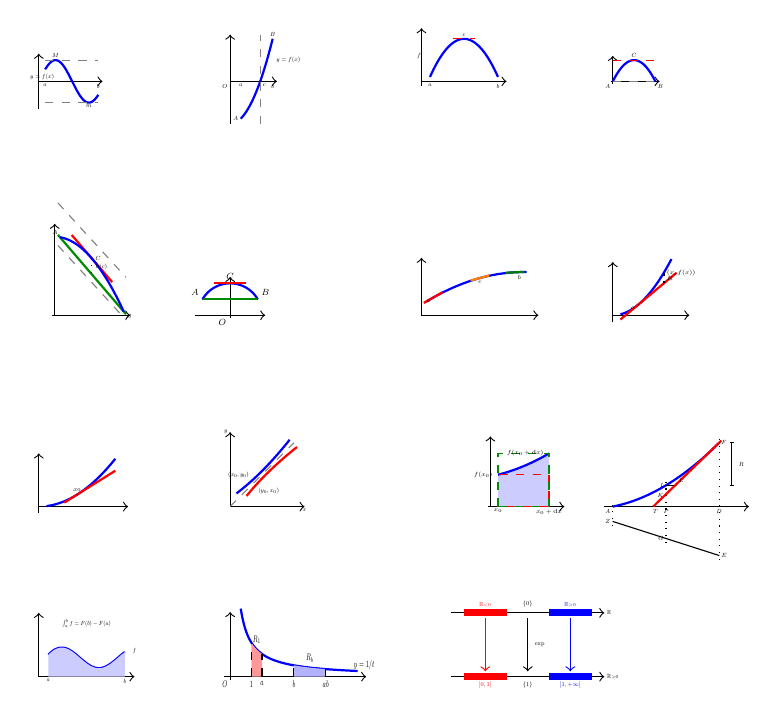
\begin{tikzpicture}[scale=0.27, transform shape, font=\footnotesize]
		
		% ================ ROW 1 ================
		
		% (a) EVT
		\begin{scope}[shift={(0,0)}]
		\draw[->] (0,-1.3) -- (0,0) -- (3,0);
		\draw[->] (0,0) -- (0,1.3);
		\draw[blue,thick,domain=0.3:2.8,samples=80,smooth] plot (\x,{sin(2*\x r)});
		\draw[dashed,gray] (0.3,1) -- (2.8,1);
		\draw[dashed,gray] (0.3,-1) -- (2.8,-1);
		\fill (0.785,1) circle (0.4pt);  \node[above] at (0.785,1) {$M$};
		\fill (2.356,-1) circle (0.4pt); \node[below] at (2.356,-1) {$m$};
		\node[below] at (0.3,0) {$a$};   \node[below] at (2.8,0) {$b$};
		\node[left] at (0.85,0.2) {$y=f(x)$};
		\end{scope}
		
		% (b) IVT
		\begin{scope}[shift={(9,0)}]
		\draw[->] (0,-2) -- (0,0) -- (2.2,0);
		\draw[->] (0,0) -- (0,2.2);
		\draw[blue,thick,domain=0.5:2,samples=60,smooth] plot (\x,{\x*\x-2});
		\draw[dotted] (0,0) -- (2.1,0);
		\draw[dashed,gray] (1.414,-2) -- (1.414,2.2);
		\fill (0.5,-1.75) circle (0.4pt); \node[left] at (0.5,-1.75) {$A$};
		\fill (2,2) circle (0.4pt);       \node[above] at (2,2) {$B$};
		\fill (1.414,0) circle (0.4pt);   \node[below right] at (1.414,0) {$c$};
		\node[below] at (0.5,0) {$a$};    \node[below] at (2,0) {$b$};
		\node[below left] at (0,0) {$O$};
		\node[right] at (2.05,1) {$y=f(x)$};
		\end{scope}
		
		% (c) Fermat
		\begin{scope}[shift={(18,0)}]
		\draw[->] (0,0) -- (4,0);
		\draw[->] (0,-0.2) -- (0,2.5);
		\draw[blue,thick,domain=0.4:3.6,samples=60,smooth] plot (\x,{2-0.7*(\x-2)*(\x-2)});
		\draw[dashed,red] (1.5,2) -- (2.5,2);
		\fill (2,2) circle (0.4pt); \node[above] at (2,2) {$c$};
		\node[below] at (0.4,0) {$a$}; \node[below] at (3.6,0) {$b$};
		\node[left] at (0.1,1.2) {$f$};
		\end{scope}
		
		% (d) Rolle
		\begin{scope}[shift={(27,0)}]
		\draw[->] (-0.1,0) -- (2.2,0); \draw[->] (0,-0.1) -- (0,1.2);
		\draw[blue,thick,domain=0:2,samples=80] plot (\x,{\x*(2-\x)});
		\draw[dashed,gray] (0,0)--(2,0); \draw[dashed,red] (0,1)--(2,1);
		\fill (0,0) circle (0.4pt); \node[below left] at (0,0) {$A$};
		\fill (2,0) circle (0.4pt); \node[below right] at (2,0) {$B$};
		\fill (1,1) circle (0.4pt); \node[above] at (1,1) {$C$};
		\end{scope}
		
		% ================ ROW 2 ================
		
		% (e) MVT sliding tangent
		\begin{scope}[shift={(0,-11)}]
		\draw[->] (0.6,0) -- (4.3,0); \draw[->] (0.75,0) -- (0.75,4.3);
		\draw[dashed,gray] (0.9,3.283)--(4.1,-0.217); \draw[dashed,gray] (0.9,5.283)--(4.1,1.783);
		\draw[green!55!black,thick] (0.9,3.783)--(4.1,0.05);
		\draw[red,thick] (1.55,3.775)--(3.45,1.559);
		\draw[blue,thick,domain=1:4,samples=120,smooth] plot (\x,{-\x*\x/3+\x/2+3.5});
		\fill (1,3.667) circle (0.4pt); \node[above left] at (1,3.667) {$A$};
		\fill (4,0.167) circle (0.4pt); \node[below right] at (4,0.167) {$B$};
		\fill (2.5,2.667) circle (0.4pt); \node[right] at (2.55,2.667) {$C$};
		\draw[dotted,blue!70!black] (2.5,2.667) -- (2.5,1.917);
		\node[right] at (2.55,2.29) {$h(c)$};
		\end{scope}
		
		% (f) Cauchy MVT
		\begin{scope}[shift={(9,-11)},xscale=1.5,yscale=1.5]
		\draw[->] (-1.1,0) -- (1.1,0); \draw[->] (0,-0.1) -- (0,1.2);
		\draw[blue,thick,domain=0.5236:2.618,samples=100,smooth] plot ({cos(\x r)},{sin(\x r)});
		\draw[green!55!black,thick] (-0.866,0.5)--(0.866,0.5);
		\draw[red,thick] (-0.5,1)--(0.5,1);
		\fill (-0.866,0.5) circle (0.4pt); \node[above left] at (-0.866,0.5) {$A$};
		\fill (0.866,0.5) circle (0.4pt); \node[above right] at (0.866,0.5) {$B$};
		\fill (0,1) circle (0.4pt); \node[above] at (0,1) {$C$};
		\node[below left] at (0,0) {$O$};
		\end{scope}
		
		% (g) Darboux
		\begin{scope}[shift={(18,-11)},xscale=1.1]
		\draw[->] (0,0) -- (5,0); \draw[->] (0,0) -- (0,2.7);
		\draw[blue,thick,domain=0.2:4.5,samples=100] plot (\x,{0.5+0.7*\x-0.08*\x*\x});
		\draw[red,thick] (0.1,0.58)--(0.9,1.08);
		\draw[orange,thick] (2.1,1.63)--(2.9,1.87);
		\draw[green!50!black,thick] (3.6,2.00)--(4.4,2.04);
		\fill (0.5,0.83) circle (0.4pt); \node[below left] at (0.5,0.83) {$a$};
		\fill (2.5,1.75) circle (0.4pt); \node[below] at (2.5,1.75) {$c$};
		\fill (4,2.02) circle (0.4pt); \node[below right] at (4,2.02) {$b$};
		\end{scope}
		
		% (h) Taylor (n=1)
		\begin{scope}[shift={(27,-11)},xscale=1.2]
		\draw[->] (0,0) -- (3,0); \draw[->] (0,-0.3) -- (0,2.5);
		\draw[blue,thick,domain=0.3:2.3,samples=60] plot (\x,{\x*\x/2});
		\draw[red,thick] (0.3,-0.2)--(2.5,2.0);
		\fill (1,0.5) circle (0.4pt); \node[below left] at (1,0.5) {$a$};
		\fill (2,2) circle (0.4pt); \node[right] at (2,2) {$(x,f(x))$};
		\fill (2,1.5) circle (0.4pt);
		\draw[dotted,thick] (2,1.5)--(2,2);
		\node[right] at (2,1.75) {$R$};
		\end{scope}
		
		% ================ ROW 3 ================
		
		% (i) Convexity
		\begin{scope}[shift={(0,-20)},xscale=1.2]
		\draw[->] (0,0) -- (3.5,0); \draw[->] (0,-0.3) -- (0,2.5);
		\draw[blue,thick,domain=0.3:3,samples=60] plot (\x,{\x*\x/4});
		\draw[red,thick] (1,0.1875)--(3,1.6875);
		\fill (1.5,0.5625) circle (0.4pt); \node[above] at (1.5,0.5625) {$x_0$};
		\end{scope}
		
		% (j) Inverse function
		\begin{scope}[shift={(9,-20)}]
		\draw[->] (0,0) -- (3.5,0) node[below] {$x$};
		\draw[->] (0,0) -- (0,3.5) node[left] {$y$};
		\draw[dashed,gray] (0,0)--(3,3);
		\draw[blue,thick,domain=0.3:2.8,samples=80] plot (\x,{0.4+0.7*\x+0.1*\x*\x});
		\draw[red,thick,domain=0.5:2.8,samples=80] plot ({0.4+0.7*\x+0.1*\x*\x},{\x});
		\fill (1,1.2) circle (0.4pt); \node[above left] at (1,1.2) {$(x_0,y_0)$};
		\fill (1.2,1) circle (0.4pt); \node[below right] at (1.2,1) {$(y_0,x_0)$};
		\end{scope}
		
		% (k) Barrow area inequality
		\begin{scope}[shift={(18,-20)},xscale=1.2,yscale=1.0]
		\draw[->] (2.6,0) -- (5.6,0); \draw[->] (2.7,0) -- (2.7,3.3);
		\fill[blue!20] (3,0) -- plot[domain=3:5,samples=60] (\x,{1.5+0.3*(\x-3)+0.1*(\x-3)*(\x-3)}) -- (5,0) -- cycle;
		\draw[blue,thick,domain=3:5,samples=60,smooth] plot (\x,{1.5+0.3*(\x-3)+0.1*(\x-3)*(\x-3)});
		\draw[dashed,red] (3,0) rectangle (5,1.5);
		\draw[dashed,green!55!black] (3,0) rectangle (5,2.5);
		\fill (3,0) circle (0.4pt); \node[below] at (3,0) {$x_0$};
		\fill (5,0) circle (0.4pt); \node[below] at (5,0) {$x_0+\mathrm{d}x$};
		\node[left] at (2.9,1.5) {$f(x_0)$};
		\node[left] at (4.9,2.5) {$f(x_0+\mathrm{d}x)$};
		\end{scope}
		
		% (l) Barrow's Fig. 109
		\begin{scope}[shift={(27,-20)}]
		\draw[->] (-0.4,0) -- (6.4,0);
		\draw[dotted] (0,-0.9) -- (0,0.3);
		\draw[dotted] (2.5,-1.7) -- (2.5,1.3);
		\draw[dotted] (5,-2.5) -- (5,3.4);
		\draw plot[smooth,tension=0.7] coordinates {(0,-0.7) (2.5,-1.5) (5,-2.3)};
		\draw[blue,thick,domain=0:5,samples=100,smooth] plot (\x,{0.08*\x*\x+0.2*\x});
		\draw[red,thick] (1.9,0)--(5.1,3.1);
		\draw[dashed] (2.5,1) -- (3,1);
		\fill (0,0) circle (0.4pt);    \node[below left]  at (0,0)    {$A$};
		\fill (2,0) circle (0.4pt);    \node[below]       at (2,0)    {$T$};
		\fill (2.5,0) circle (0.4pt);  \node[below]       at (2.5,0)  {$P$};
		\fill (5,0) circle (0.4pt);    \node[below]       at (5,0)    {$D$};
		\fill (0,-0.7) circle (0.4pt); \node[left]        at (0,-0.7) {$Z$};
		\fill (2.5,-1.5) circle (0.4pt);\node[left]       at (2.5,-1.5){$G$};
		\fill (5,-2.3) circle (0.4pt); \node[right]       at (5,-2.3) {$E$};
		\fill (2.5,1) circle (0.4pt);  \node[left]        at (2.5,1)  {$I$};
		\fill (2.5,0.5) circle (0.4pt);\node[left]        at (2.5,0.5){$K$};
		\fill (3,1) circle (0.4pt);    \node[above right] at (3,1)    {$L$};
		\fill (5,3) circle (0.4pt);    \node[right]       at (5,3)    {$F$};
		\draw (5.5,1) -- (5.7,1); \draw (5.5,3) -- (5.7,3); \draw (5.6,1) -- (5.6,3);
		\node[right] at (5.8,2) {$R$};
		\end{scope}
		
		% ================ ROW 4 ================
		
		% (m) Second FTC
		\begin{scope}[shift={(0,-28)},xscale=0.9]
		\draw[->] (0,0) -- (5,0); \draw[->] (0,0) -- (0,3);
		\draw[blue,thick,domain=0.5:4.5,samples=80] plot (\x,{0.5+0.6*sin(\x*1.5 r)+0.5*sin(\x*0.5 r)});
		\fill[blue!20] (0.5,0) -- plot[domain=0.5:4.5,samples=80] (\x,{0.5+0.6*sin(\x*1.5 r)+0.5*sin(\x*0.5 r)}) -- (4.5,0) -- cycle;
		\node[above] at (2.5,2.2) {$\int_a^b f = F(b)-F(a)$};
		\node[below] at (0.5,0) {$a$}; \node[below] at (4.5,0) {$b$};
		\node[right] at (4.8,1.2) {$f$};
		\end{scope}
		
		% (n) Hyperbolic similarity (log)
		\begin{scope}[shift={(9,-28)},xscale=1.0,yscale=1.6]
		\draw[->] (-0.3,0) -- (6.4,0); \draw[->] (0,-0.1) -- (0,1.9);
		\draw[blue,thick,domain=0.5:6,samples=150,smooth] plot (\x,{1/\x});
		\fill[red!40] (1,0) -- plot[domain=1:1.5,samples=30] (\x,{1/\x}) -- (1.5,0) -- cycle;
		\fill[blue!30] (3,0) -- plot[domain=3:4.5,samples=30] (\x,{1/\x}) -- (4.5,0) -- cycle;
		\draw[dashed] (1,0) -- (1,1); \draw[dashed] (1.5,0) -- (1.5,0.667);
		\draw[dashed] (3,0) -- (3,0.333); \draw[dashed] (4.5,0) -- (4.5,0.222);
		\node[below] at (1,0) {$1$}; \node[below] at (1.5,0) {$a$};
		\node[below] at (3,0) {$b$}; \node[below] at (4.5,0) {$ab$};
		\node[above] at (1.25,0.85) {$R_1$};
		\node[above] at (3.75,0.30) {$R_b$};
		\node[right] at (5.7,0.35) {$y=1/t$};
		\node[below left] at (0,0) {$O$};
		\end{scope}
		
	% (o) Image exp / ln
	\begin{scope}[shift={(20,-25)}]
	% Top axis: domain R
	\draw[->] (-0.6,0) -- (6.6,0) node[right] {$\R$};
	\draw[red,line width=2.5pt] (0,0)--(2,0);
	\draw[blue,line width=2.5pt] (4,0)--(6,0);
	\fill (3,0) circle (0.5pt);
	\node[above=4pt] at (1,0) {\textcolor{red}{$\R_{<0}$}};
	\node[above=4pt] at (3,0) {$\{0\}$};
	\node[above=4pt] at (5,0) {\textcolor{blue}{$\R_{>0}$}};
	% exp arrows
	\draw[->,red]  (1,-0.25) -- (1,-2.75);
	\draw[->]      (3,-0.25) -- (3,-2.75);
	\draw[->,blue] (5,-0.25) -- (5,-2.75);
	\node[right=6pt] at (3,-1.5) {$\exp$};
	% Bottom axis: codomain R_{>0}
	\draw[->] (-0.6,-3) -- (6.6,-3) node[right] {$\R_{>0}$};
	\draw[red,line width=2.5pt] (0,-3)--(2,-3);
	\draw[blue,line width=2.5pt] (4,-3)--(6,-3);
	\fill (3,-3) circle (0.5pt);
	\node[below=4pt] at (1,-3) {\textcolor{red}{${]}0,1[$}};
	\node[below=4pt] at (3,-3) {$\{1\}$};
	\node[below=4pt] at (5,-3) {\textcolor{blue}{${]}1,+\infty[$}};
	\end{scope}
		\end{tikzpicture}}

\end{figure}
\newpage
\thispagestyle{empty}
\tableofcontents
\newpage
\pagestyle{plain}\pagenumbering{arabic}

\section*{Introduction}
\label{sec:introduction}
\setstretch{1.3}
\noindent Barrow's \emph{Geometrical Lectures} (1670) give the first calculus textbook and the first geometric proof of the Fundamental Theorem of Calculus; see \cite{Barrow1916,Lopez2026}.

Part~I develops the classical theorems of single-variable real analysis --- EVT\comma IVT\comma Fermat\comma Rolle\comma MVT and its refinements\comma convexity\comma inverse function\comma the Fundamental Theorems of Calculus\comma and the $\ln$/$\exp$ addition and image theorems --- in Barrow's geometric idiom\comma with figures and geometric proofs.

Part~II classifies each theorem in reverse mathematics. Every axiom\comma postulate\comma definition and statement of Part~I reappears as a tagged entry with a dependency table and an exact strength. Classification: all entries are $\textsf{RCA}_0$ except IVT\comma EVT\comma Darboux\comma and the weighted MVT\comma which are $\textsf{WKL}_0$. No entry uses Cauchy completeness or any form of Choice \cite{Propp2012,Jech1973}. Coding conventions are in \S\ref{sec:coding}.

\part{A Geometric Development of Classical Real Analysis}

\noindent Following Barrow \cite[Lecture~X, \S 11]{Barrow1916}\comma we state and prove the classical theorems in Barrow's geometric idiom. See \cite{Lopez2026} for commentary.

\section{Axioms, definitions and geometric conventions}
\label{sec:conventions}

Let $[a\comma b]\subseteq\R$ and let $f\colon[a\comma b]\to\R$ be continuous. The \emph{area function} is
\begin{equation}\label{eq:area}
A_a^x:=\text{(signed) area of }\{(t\comma y): a\le t\le x\comma\ 0\le y\le f(t)\}\comma
\end{equation}
with Barrow's orientation
\begin{equation}\label{eq:oriented-area}
A_x^{x}=0\comma\qquad A_x^{x+\mathrm{d}x}=-A_{x+\mathrm{d}x}^{x}\quad(\mathrm{d}x<0).
\end{equation}
The curve $u\mapsto A_a^u$ is Barrow's $AIF$; $f(x_0)$ is his $DE$; the unit is his $R$.

\paragraph{$\textsf{\underline{Differentiability.}}$}\text{\ } $f$ is differentiable at $x$ if
\begin{equation}\label{eq:diff}
\lim_{h\to 0}(f(x+h)-f(x))/h=f'(x)
\end{equation}
exists.

\paragraph{\textsf{\underline{Tangency (little-\textit{o} form).}}}
$G$ is differentiable at $x_0$ with tangent $L(u)=m(u-x_0)+G(x_0)$ iff
\begin{equation}\label{eq:little-o}
G(x_0+\Delta x)=G(x_0)+m\,\Delta x+\Delta x\cdot o(\Delta x)\quad(\Delta x\to0)\comma
\end{equation}
in which case $G'(x_0)=m$; cf.\ \cite[Theorem~2]{Lopez2026}.

\paragraph{$\textsf{\underline{Lin-Integ.}}$}\text{\ }
\begin{equation}\label{eq:lin-int}
\forall u\comma v\comma w\in[a\comma b]:\ A_u^w=A_u^v+A_v^w.
\end{equation}

\paragraph{$\textsf{\underline{Int-Mono.}}$}\text{\ }
\begin{equation}\label{eq:int-mono}
f\le g\ \text{on}\ [a\comma b]\Rightarrow\int_a^b f\le\int_a^b g.
\end{equation}

\paragraph{$\textsf{\underline{Similarity.}}$}\text{\ } For $b>0$\comma
\begin{equation}\label{eq:similarity}
\int_b^{ab} h(t)\,\mathrm{d}t=\int_1^a h(bu)\,b\,\mathrm{d}u.
\end{equation}

\paragraph{$\textsf{\underline{Inv-Cont.}}$}\text{\ }
\begin{equation}\label{eq:inv-cont}
t\mapsto1/t\in C^0(\R_{>0}).
\end{equation}

\paragraph{$\textsf{\underline{Image-Union.}}$}\text{\ }
\begin{equation}\label{eq:image-union}
f(A\cup B)=f(A)\cup f(B).
\end{equation}

\paragraph{$\textsf{\underline{Product\,rule.}}$}\text{\ }
\begin{equation}\label{eq:product-rule}
(fg)'(x)=f'(x)g(x)+f(x)g'(x).
\end{equation}

\paragraph{$\textsf{\underline{Chain\,rule.}}$}\text{\ }
\begin{equation}\label{eq:chain-rule}
(f\circ g)'(x)=f'(g(x))\,g'(x).
\end{equation}

\paragraph{$\textsf{\underline{Sign-Law.}}$}\text{\ }
\begin{equation}\label{eq:sign-law}
\forall u>0:\ \bigl(\ln u<0\iff u<1\bigr)\wedge\bigl(\ln u=0\iff u=1\bigr)\wedge\bigl(\ln u>0\iff u>1\bigr).
\end{equation}

\paragraph{$\textsf{\underline{Ln-Bij.}}$}\text{\ } $\ln:\R_{>0}\to\R$ is bijective; $\exp:=\ln^{-1}:\R\to\R_{>0}$\comma i.e.
\begin{equation}\label{eq:ln-bij}
\exp:=\ln^{-1}:\R\to\R_{>0}.
\end{equation}

\paragraph{$\textsf{\underline{Barrow-tangency.}}$}\text{\ } Let $G$ be differentiable at $x_0$\comma and let $L(u)=m(u-x_0)+G(x_0)$ be the line through $(x_0\comma G(x_0))$ of slope $m$. If $L\le G$ (or $L\ge G$) on a punctured neighbourhood of $x_0$\comma then
\begin{equation}\label{eq:barrow-tangency}
m=G'(x_0).
\end{equation}
\footnote{The two-sided hypothesis strengthens Barrow's one-sided criterion\comma which fails at inflections \cite{Lopez2026}. Every use in Part~I is in a convex or concave setting\comma where the two-sided hypothesis holds.}

\section{Statements of the classical theorems}

\subsection{Topological theorems}

\begin{theorem}[Extreme Value Theorem]
	\label{thm:evt}
	If $f:[a\comma b]\to\R$ is continuous\comma then
	\begin{equation}\label{eq:evt}
	\exists x_{\max}\comma x_{\min}\in[a\comma b]\comma\ \forall x\in[a\comma b]:\ f(x_{\min})\le f(x)\le f(x_{\max}).
	\end{equation}
\end{theorem}

\begin{theorem}[Intermediate Value Theorem]
	\label{thm:ivt}
	If $f:[a\comma b]\to\R$ is continuous and $f(a)f(b)<0$\comma then
	\begin{equation}\label{eq:ivt}
	\exists c\in(a\comma b):\ f(c)=0.
	\end{equation}
\end{theorem}

\subsection{Differentiation theorems}

\begin{theorem}[Fermat]
	\label{thm:fermat}
	If $f$ has a local extremum at $c\in(a\comma b)$ and is differentiable at $c$\comma then
	\begin{equation}\label{eq:fermat}
	f'(c)=0.
	\end{equation}
\end{theorem}

\begin{theorem}[Rolle]
	\label{thm:rolle}
	If $f$ is continuous on $[a\comma b]$\comma differentiable on $(a\comma b)$\comma and $f(a)=f(b)$\comma then $\exists c\in(a\comma b):\,f'(c)=0$.
\end{theorem}

\begin{theorem}[Mean-Value Theorem]
	\label{thm:mvt}
	If $f$ is continuous on $[a\comma b]$ and differentiable on $(a\comma b)$\comma then
	\begin{equation}\label{eq:mvt}
	\exists c\in(a\comma b):\ f'(c)=\frac{f(b)-f(a)}{b-a}.
	\end{equation}
	Geometrically\comma $d_c\parallel d_{a\comma b}$.
\end{theorem}

\begin{theorem}[Constant-function]
	\label{thm:const}
	If $f$ is continuous on $[a\comma b]$\comma differentiable on $(a\comma b)$\comma and $f'=0$ on $(a\comma b)$\comma then
	\begin{equation}\label{eq:const}
	f(x)=f(a)\quad\text{for all }x\in[a\comma b].
	\end{equation}
\end{theorem}

\begin{theorem}[Monotonicity]
	\label{thm:monotone}
	If $f$ is continuous on $[a\comma b]$\comma differentiable on $(a\comma b)$\comma and $f'\ge0$ (resp.\ $f'>0$)\comma then
	\begin{equation}\label{eq:monotone}
	x<y\Rightarrow f(x)\le f(y)\quad\text{(resp.\ }f(x)<f(y)\text{)}
	\end{equation}
	for all $x\comma y\in[a\comma b]$.
\end{theorem}

\begin{theorem}[Cauchy MVT]
	\label{thm:cauchy-mvt}
	If $f\comma g$ are continuous on $[a\comma b]$\comma differentiable on $(a\comma b)$\comma and $g'\ne0$ on $(a\comma b)$\comma then
	\begin{equation}\label{eq:cauchy-mvt}
	\exists c\in(a\comma b):\ \frac{f'(c)}{g'(c)}=\frac{f(b)-f(a)}{g(b)-g(a)}.
	\end{equation}
\end{theorem}

\begin{theorem}[Darboux]
	\label{thm:darboux}
	If $f$ is differentiable on $[a\comma b]$ and $f'(a)<\lambda<f'(b)$\comma then
	\begin{equation}\label{eq:darboux}
	\exists c\in(a\comma b):\ f'(c)=\lambda.
	\end{equation}
\end{theorem}

\begin{theorem}[L'H\^opital]
	\label{thm:lhopital}
	Let $f\comma g$ be differentiable near $a$\comma with $f(a)=g(a)=0$\comma $g'\ne0$ near $a$\comma and $\lim_{x\to a}f'(x)/g'(x)=L$. Then
	\begin{equation}\label{eq:lhopital}
	\lim_{x\to a}f(x)/g(x)=L.
	\end{equation}
\end{theorem}

\begin{theorem}[Taylor\comma Lagrange remainder]
	\label{thm:taylor}
	If $f$ is $(n+1)$-times differentiable on an interval containing $a$ and $x$\comma then
	\begin{equation}\label{eq:taylor}
	\exists c\ \text{between}\ a\comma x:\ f(x)=\sum_{k=0}^{n}\frac{f^{(k)}(a)}{k!}(x-a)^{k}+\frac{f^{(n+1)}(c)}{(n+1)!}(x-a)^{n+1}.
	\end{equation}
\end{theorem}

\begin{theorem}[Convexity]
	\label{thm:convexity}
	If $f$ is twice differentiable on $[a\comma b]$ and $f''\ge0$ on $(a\comma b)$\comma then
	\begin{equation}\label{eq:convexity}
	f(x)\ge f(x_0)+f'(x_0)(x-x_0)\quad\text{for all }x\comma x_0\in[a\comma b].
	\end{equation}
\end{theorem}

\begin{theorem}[Inverse function]
	\label{thm:inverse}
	If $f:I\to\R$ is continuous and strictly monotone on $I$\comma $x_0$ lies in the interior $I^\circ$ of $I$\comma and $f$ is differentiable at $x_0$ with $f'(x_0)\ne0$\comma then $f^{-1}$ is differentiable at $y_0=f(x_0)$ with
	\begin{equation}\label{eq:inverse}
	(f^{-1})'(y_0)=1/f'(x_0).
	\end{equation}
\end{theorem}

\subsection{Integration theorems}

\begin{lemma}[Barrow's area inequality]
	\label{lem:barrow-area}
	If $f$ is continuous and increasing on $[a\comma b]$ and $x_0\comma x_0+\mathrm{d}x\in[a\comma b]$\comma $\mathrm{d}x\ne0$\comma then
	\begin{equation}\label{eq:barrow-area}
	f(x_0)\,\mathrm{d}x\le A_{x_0}^{x_0+\mathrm{d}x}\le f(x_0+\mathrm{d}x)\,\mathrm{d}x,
	\end{equation}
	and both inequalities are strict when $f$ is strictly increasing on the interval with endpoints $x_0$ and $x_0+\mathrm{d}x$.
\end{lemma}

\begin{lemma}[MVT for integrals]
	\label{lem:mvt-int}
	If $f$ is continuous on $[a\comma b]$ and $x_0\comma x_0+\mathrm{d}x\in[a\comma b]$\comma $\mathrm{d}x\ne0$\comma then
	\begin{equation}\label{eq:mvt-int}
	\exists\theta\ \text{between}\ x_0\comma x_0+\mathrm{d}x:\ A_{x_0}^{x_0+\mathrm{d}x}=f(\theta)\,\mathrm{d}x.
	\end{equation}
\end{lemma}

\begin{theorem}[First FTC; Barrow]
	\label{thm:fftc}
	If $f$ is continuous on $[a\comma b]$\comma then
	\begin{equation}\label{eq:fftc}
	\frac{d}{dx}\int_a^x f=f(x)
	\end{equation}
	for every $x\in(a\comma b)$\comma with one-sided versions at $a\comma b$.
\end{theorem}

\begin{theorem}[Second FTC]
	\label{thm:second-ftc}
	If $F$ is differentiable on $[a\comma b]$ and $F'=f$ is continuous\comma then
	\begin{equation}\label{eq:second-ftc}
	\int_a^b f=F(b)-F(a).
	\end{equation}
\end{theorem}

\begin{theorem}[Integration by parts]
	\label{thm:ibp}
	If $f\comma g\in C^1([a\comma b])$\comma then
	\begin{equation}\label{eq:ibp}
	\int_a^b fg'=[fg]_a^b-\int_a^b f'g.
	\end{equation}
\end{theorem}

\begin{theorem}[Change of variables]
	\label{thm:subst}
	If $g\in C^1([a\comma b])$ and $f$ is continuous on $g([a\comma b])$\comma then
	\begin{equation}\label{eq:subst}
	\int_{g(a)}^{g(b)}f=\int_a^b f(g)\,g'.
	\end{equation}
\end{theorem}

\begin{theorem}[Weighted MVT]
	\label{thm:weighted-mvt}
	If $f$ is continuous on $[a\comma b]$\comma $w\ge0$ is Riemann integrable\comma and $\int_a^b w>0$\comma then
	\begin{equation}\label{eq:weighted-mvt}
	\exists c\in[a\comma b]:\ \int_a^b fw=f(c)\int_a^b w.
	\end{equation}
\end{theorem}

\subsection{The logarithm and the exponential}

\begin{theorem}[Log\,-Property]
	\label{thm:log}
	With $\ln(x):=\int_1^x \mathrm{d}t/t$ ($x>0$)\comma
	\begin{equation}\label{eq:log}
	\forall a\comma b>0:\ \ln(a)+\ln(b)=\ln(ab).
	\end{equation}
\end{theorem}

\begin{theorem}[Exp\,-Property]
	\label{thm:exp}
	With $\exp:=\ln^{-1}$\comma
	\begin{equation}\label{eq:exp}
	\forall u\comma v\in\R:\ \exp(u)\exp(v)=\exp(u+v).
	\end{equation}
\end{theorem}

\begin{theorem}[Exp\,-Image]
	\label{thm:image}
	\begin{equation}\label{eq:image}
	\exp(\R)=\R_{>0}\comma\qquad \ln(\R_{>0})=\R.
	\end{equation}
\end{theorem}

\section{Geometrical proofs}

\subsection{Topological theorems}

\begin{proof}[Proof of Theorem~\ref{thm:evt}]
	$S=f([a\comma b])$ is nonempty and bounded; let $M=\sup S$\comma $m=\inf S$. Were $M$ unattained\comma $1/(M-f)$ would be continuous and unbounded on $[a\comma b]$; contradiction. So $M=f(x_{\max})$; symmetrically $m=f(x_{\min})$\comma giving \eqref{eq:evt}.\hfill$\square$
\end{proof}

\begin{figure}[H]
	\centering
	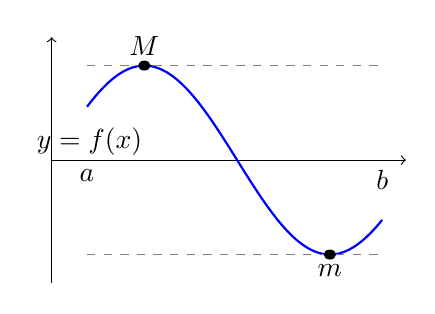
\begin{tikzpicture}[xscale=1.5,yscale=1.2]
	\draw[->] (0,-1.3) -- (0,0) -- (3,0); \draw[->] (0,0) -- (0,1.3);
	\draw[blue,thick,domain=0.3:2.8,samples=100,smooth] plot (\x,{sin(2*\x r)});
	\draw[dashed,gray] (0.3,1)--(2.8,1); \draw[dashed,gray] (0.3,-1)--(2.8,-1);
	\fill (0.785,1) circle (1.5pt); \node[above] at (0.785,1) {$M$};
	\fill (2.356,-1) circle (1.5pt); \node[below] at (2.356,-1) {$m$};
	\node[below] at (0.3,0) {$a$}; \node[below] at (2.8,0) {$b$};
	\node[left] at (0.85,0.2) {$y=f(x)$};
	\end{tikzpicture}
	\caption{EVT.}
	\label{fig:evt}
\end{figure}

\begin{proof}[Proof of Theorem~\ref{thm:ivt}]
	Assume $f(a)<0<f(b)$ and let $c=\sup\{x\in[a\comma b]:f(x)<0\}$. By continuity $f(c)\le 0$; if $f(c)<0$ then $f<0$ on a neighbourhood of $c$ intersected with $[a\comma b]$, contradicting the definition of $c$ as an upper bound; hence \eqref{eq:ivt} holds.\hfill$\square$
\end{proof}

\begin{figure}[H]
	\centering
	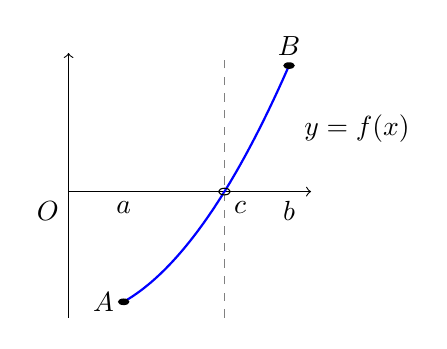
\begin{tikzpicture}[xscale=1.4,yscale=0.8]
	\draw[->] (0,-2) -- (0,0) -- (2.2,0); \draw[->] (0,0) -- (0,2.2);
	\draw[blue,thick,domain=0.5:2,samples=80,smooth] plot (\x,{\x*\x-2});
	\draw[dotted] (0,0)--(2.1,0); \draw[dashed,gray] (1.414,-2)--(1.414,2.2);
	\fill (0.5,-1.75) circle (1.5pt); \node[left] at (0.5,-1.75) {$A$};
	\fill (2,2) circle (1.5pt); \node[above] at (2,2) {$B$};
	\draw (1.414,0) circle (1.5pt); \node[below right] at (1.414,0) {$c$};
	\node[below] at (0.5,0) {$a$}; \node[below] at (2,0) {$b$};
	\node[below left] at (0,0) {$O$};
	\node[right] at (2.05,1) {$y=f(x)$};
	\end{tikzpicture}
	\caption{IVT.}
	\label{fig:ivt}
\end{figure}

\subsection{Differentiation theorems}

\begin{proof}[Proof of Theorem~\ref{thm:fermat}]
	If $c$ is a local max: $(f(c+h)-f(c))/h\le0$ for $h>0^+$ gives $f'(c)\le0$; for $h<0^-$\comma $\ge0$ gives $f'(c)\ge0$. So $f'(c)=0$.\hfill$\square$
\end{proof}

\begin{figure}[H]
	\centering
	\begin{tikzpicture}[xscale=1.2]
	\draw[->] (0,0) -- (4,0); \draw[->] (0,-0.2) -- (0,2.5);
	\draw[blue,thick,domain=0.4:3.6,samples=80] plot (\x,{2-0.7*(\x-2)*(\x-2)});
	\draw[dashed,red] (1.5,2)--(2.5,2); \fill (2,2) circle (1.5pt); \node[above] at (2,2) {$c$};
	\node[below] at (0.4,0) {$a$}; \node[below] at (3.6,0) {$b$};
	\node[left] at (0.1,1.2) {$f$};
	\end{tikzpicture}
	\caption{Fermat.}
	\label{fig:fermat}
\end{figure}

\begin{proof}[Proof of Theorem~\ref{thm:rolle}]
	By EVT\comma $f$ attains $M\comma m$. If $M=m$\comma $f$ constant. Otherwise\comma $f(a)=f(b)$ forces an interior extremum $c$; Fermat gives $f'(c)=0$.\hfill$\square$
\end{proof}

\begin{figure}[H]
	\centering
	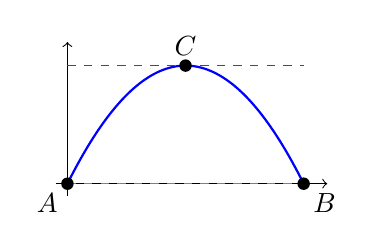
\begin{tikzpicture}[xscale=1.5,yscale=1.5]
	\draw[->] (-0.1,0) -- (2.2,0); \draw[->] (0,-0.1) -- (0,1.2);
	\draw[blue,thick,domain=0:2,samples=80] plot (\x,{\x*(2-\x)});
	\draw[dashed,gray] (0,0)--(2,0); \draw[dashed,red] (0,1)--(2,1);
	\fill (0,0) circle (1.5pt); \node[below left] at (0,0) {$A$};
	\fill (2,0) circle (1.5pt); \node[below right] at (2,0) {$B$};
	\fill (1,1) circle (1.5pt); \node[above] at (1,1) {$C$};
	\end{tikzpicture}
	\caption{Rolle.}
	\label{fig:rolle}
\end{figure}

\begin{proof}[Proof of Theorem~\ref{thm:mvt} (Barrow's sliding tangent)]
	Let $L$ be the chord line\comma $g=f-L$. Then $g(a)=g(b)=0$; by EVT\comma $g$ attains $M\comma m$.
	\emph{Case $M>0$:} maximum at $c\in(a\comma b)$; the translate $L+M$ touches $f$ at $C$ and lies above; by concave Barrow-tangency\comma slope $=f'(c)=L'(c)=(f(b)-f(a))/(b-a)$.
	\emph{Case $M=0$:} if $f=L$ identically\comma trivial; otherwise $m<0$ with minimum at interior $c$ and the same argument via convex Barrow-tangency. So $d_c\parallel d_{a\comma b}$.\hfill$\square$
\end{proof}

\begin{figure}[H]
	\centering
	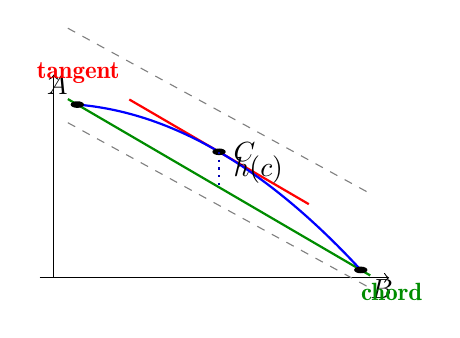
\begin{tikzpicture}[xscale=1.2,yscale=0.6]
	\draw[->] (0.6,0) -- (4.3,0); \draw[->] (0.75,0) -- (0.75,4.3);
	\draw[dashed,gray] (0.9,3.283)--(4.1,-0.217); \draw[dashed,gray] (0.9,5.283)--(4.1,1.783);
	\draw[green!55!black,thick] (0.9,3.783)--(4.1,0.05);
	\draw[red,thick] (1.55,3.775)--(3.45,1.559);
	\draw[blue,thick,domain=1:4,samples=120,smooth] plot (\x,{-\x*\x/3+\x/2+3.5});
	\fill (1,3.667) circle (2pt); \node[above left] at (1,3.667) {$A$};
	\fill (4,0.167) circle (2pt); \node[below right] at (4,0.167) {$B$};
	\fill (2.5,2.667) circle (2pt); \node[right] at (2.55,2.667) {$C$};
	\draw[dotted,blue!70!black,thick] (2.5,2.667) -- (2.5,1.917);
	\node[right] at (2.55,2.29) {$h(c)$};
	\node[below right] at (3.9,0.10) {\textcolor{green!55!black}{\small chord}};
	\node[above left] at (1.55,3.90) {\textcolor{red}{\small tangent}};
	\end{tikzpicture}
	\caption{MVT sliding tangent.}
	\label{fig:mvt}
\end{figure}

\begin{proof}[Proof of Theorem~\ref{thm:const}]
	MVT on $[a\comma x]$: $f(x)-f(a)=f'(c)(x-a)=0$.\hfill$\square$
\end{proof}

\begin{proof}[Proof of Theorem~\ref{thm:monotone}]
	MVT on $[x_1\comma x_2]$: $f(x_2)-f(x_1)=f'(c)(x_2-x_1)$; sign of $f'(c)$ gives the result.\hfill$\square$
\end{proof}

\begin{proof}[Proof of Theorem~\ref{thm:cauchy-mvt}]
	$h:=(f(b)-f(a))g-(g(b)-g(a))f$ satisfies $h(a)=h(b)$\comma so Rolle gives $c$ with $(f(b)-f(a))g'(c)=(g(b)-g(a))f'(c)$; $g'$ and $g(b)-g(a)$ are nonzero\comma so \eqref{eq:cauchy-mvt}.\hfill$\square$
\end{proof}

\begin{figure}[H]
	\centering
	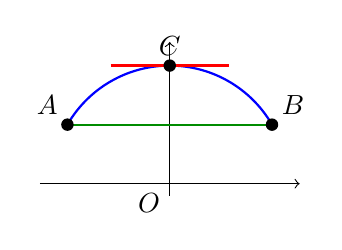
\begin{tikzpicture}[xscale=1.5,yscale=1.5]
	\draw[->] (-1.1,0) -- (1.1,0); \draw[->] (0,-0.1) -- (0,1.2);
	\draw[blue,thick,domain=0.5236:2.618,samples=100,smooth] plot ({cos(\x r)},{sin(\x r)});
	\draw[green!55!black,thick] (-0.866,0.5)--(0.866,0.5);
	\draw[red,thick] (-0.5,1)--(0.5,1);
	\fill (-0.866,0.5) circle (1.5pt); \node[above left] at (-0.866,0.5) {$A$};
	\fill (0.866,0.5) circle (1.5pt); \node[above right] at (0.866,0.5) {$B$};
	\fill (0,1) circle (1.5pt); \node[above] at (0,1) {$C$};
	\node[below left] at (0,0) {$O$};
	\end{tikzpicture}
	\caption{Cauchy MVT.}
	\label{fig:cauchy-mvt}
\end{figure}

\begin{proof}[Proof of Theorem~\ref{thm:darboux}]
	$g=f-\lambda x$ has $g'(a)<0<g'(b)$. Small $h$ gives $g(a+h)<g(a)$ and $g(b-h)<g(b)$; by EVT the minimum of $g$ is interior\comma at $c$. Fermat: $g'(c)=0$\comma i.e.\ $f'(c)=\lambda$.\hfill$\square$
\end{proof}

\begin{figure}[H]
	\centering
	\begin{tikzpicture}[xscale=1.1]
	\draw[->] (0,0) -- (5,0); \draw[->] (0,0) -- (0,2.7);
	\draw[blue,thick,domain=0.2:4.5,samples=100] plot (\x,{0.5+0.7*\x-0.08*\x*\x});
	\draw[red,thick] (0.1,0.58)--(0.9,1.08);
	\draw[orange,thick] (2.1,1.63)--(2.9,1.87);
	\draw[green!50!black,thick] (3.6,2.00)--(4.4,2.04);
	\fill (0.5,0.83) circle (1.5pt); \node[below left] at (0.5,0.83) {$a$};
	\fill (2.5,1.75) circle (1.5pt); \node[below] at (2.5,1.75) {$c$};
	\fill (4,2.02) circle (1.5pt); \node[below right] at (4,2.02) {$b$};
	\end{tikzpicture}
	\caption{Darboux.}
	\label{fig:darboux}
\end{figure}

\begin{proof}[Proof of Theorem~\ref{thm:lhopital}]
	Cauchy MVT on $[a\comma x]$: $f(x)/g(x)=f'(c_x)/g'(c_x)$; $c_x\to a$ as $x\to a^+$. Symmetric for $x\to a^-$. So the limit is $L$.\hfill$\square$
\end{proof}

\begin{proof}[Proof of Theorem~\ref{thm:taylor}]
	$P:=\sum f^{(k)}(a)(t-a)^k/k!$; choose $M$ with $f(x)=P(x)+M(x-a)^{n+1}$; $h=f-P-M(t-a)^{n+1}$ has $h^{(j)}(a)=0$\comma $h(x)=0$. Rolle $n+1$ times: $h^{(n+1)}(c)=0$\comma so $M=f^{(n+1)}(c)/(n+1)!$.\hfill$\square$
\end{proof}

\begin{figure}[H]
	\centering
	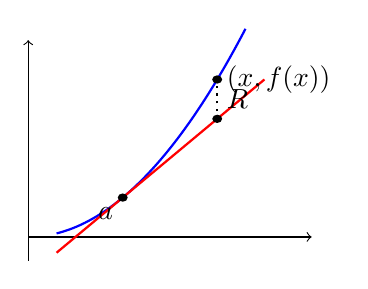
\begin{tikzpicture}[xscale=1.2]
	\draw[->] (0,0) -- (3,0); \draw[->] (0,-0.3) -- (0,2.5);
	\draw[blue,thick,domain=0.3:2.3,samples=60] plot (\x,{\x*\x/2});
	\draw[red,thick] (0.3,-0.2)--(2.5,2.0);
	\fill (1,0.5) circle (1.5pt); \node[below left] at (1,0.5) {$a$};
	\fill (2,2) circle (1.5pt); \node[right] at (2,2) {$(x,f(x))$};
	\fill (2,1.5) circle (1.5pt);
	\draw[dotted,thick] (2,1.5)--(2,2);
	\node[right] at (2,1.75) {$R$};
	\end{tikzpicture}
	\caption{Taylor ($n=1$).}
	\label{fig:taylor}
\end{figure}

\begin{proof}[Proof of Theorem~\ref{thm:convexity}]
	$g=f-f(x_0)-f'(x_0)(x-x_0)$ has $g''\ge0$; $g'$ nondecreasing and $g'(x_0)=0$\comma so $g'\le0$ before and $\ge0$ after $x_0$; with $g(x_0)=0$\comma $g\ge0$. Hence \eqref{eq:convexity}.\hfill$\square$
\end{proof}

\begin{figure}[H]
	\centering
	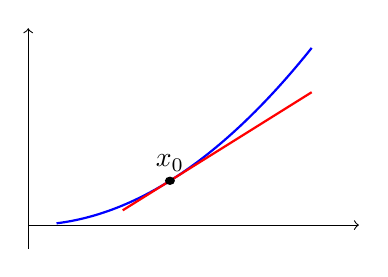
\begin{tikzpicture}[xscale=1.2]
	\draw[->] (0,0) -- (3.5,0); \draw[->] (0,-0.3) -- (0,2.5);
	\draw[blue,thick,domain=0.3:3,samples=60] plot (\x,{\x*\x/4});
	\draw[red,thick] (1,0.1875)--(3,1.6875);
	\fill (1.5,0.5625) circle (1.5pt); \node[above] at (1.5,0.5625) {$x_0$};
	\end{tikzpicture}
	\caption{Convexity.}
	\label{fig:convexity}
\end{figure}

\begin{proof}[Proof of Theorem~\ref{thm:inverse}]
	Let $c:=f'(x_0)\ne0$. Since $x_0\in I^\circ$\comma choose $\rho>0$ with $(x_0-\rho\comma x_0+\rho)\subseteq I$. \emph{Local surjectivity.} Assume without loss of generality that $f$ is strictly increasing on $I$ (the strictly decreasing case is symmetric). Choose $x_0^-\comma x_0^+\in(x_0-\rho\comma x_0+\rho)$ with $x_0^-<x_0<x_0^+$; then $f(x_0^-)<y_0<f(x_0^+)$. By the intermediate value theorem applied to the continuous function $f$ on the closed subinterval $[x_0^-\comma x_0^+]\subseteq I$\comma every $y\in(f(x_0^-)\comma f(x_0^+))$ is attained at some $x\in(x_0^-\comma x_0^+)\subseteq I$. Hence $(f(x_0^-)\comma f(x_0^+))\subseteq f(I)$ is an open neighbourhood of $y_0$\comma and $f^{-1}$ is defined on it.

	\emph{Continuity of $f^{-1}$ at $y_0$.} Differentiability of $f$ at $x_0$ gives, for some $\delta_0\in(0\comma\rho)$ and all $x$ with $|x-x_0|<\delta_0$\comma
	\[
	|f(x)-f(x_0)-c(x-x_0)|<\tfrac{|c|}{2}|x-x_0|\comma
	\]
	whence by the reverse triangle inequality $|f(x)-f(x_0)|\ge\tfrac{|c|}{2}|x-x_0|$ on the same neighbourhood. Given $\varepsilon>0$\comma set $\varepsilon':=\min(\varepsilon\comma\delta_0)$ and
	\[
	\eta:=\min\Bigl(\tfrac{|c|}{2}\varepsilon'\comma\;
	y_0-f(x_0^-)\comma\;f(x_0^+)-y_0\Bigr)>0.
	\]
	Suppose $|y-y_0|<\eta$. Since $y\in(f(x_0^-)\comma f(x_0^+))\subseteq f(I)$\comma the value $x:=f^{-1}(y)\in(x_0-\rho\comma x_0+\rho)\subseteq I$ is defined. In the case $|x-x_0|<\delta_0$\comma the bound above gives $|y-y_0|\ge\tfrac{|c|}{2}|x-x_0|$\comma so $|x-x_0|<\varepsilon'\le\varepsilon$. In the case $|x-x_0|\ge\delta_0$\comma let $x_1:=x_0+\operatorname{sgn}(x-x_0)\,\delta_0\in(x_0-\rho\comma x_0+\rho)\subseteq I$ be the point of $I$ at distance exactly $\delta_0$ from $x_0$ on the side of $x$. By strict monotonicity of $f$\comma $|y-y_0|\ge|f(x_1)-f(x_0)|$. Passing the bound $|f(u)-f(x_0)|\ge\tfrac{|c|}{2}|u-x_0|$\comma valid for $|u-x_0|<\delta_0$\comma to the limit $u\to x_1$ from inside $(x_0\comma x_1)$ (using continuity of $f$ at $x_1$) yields $|f(x_1)-f(x_0)|\ge\tfrac{|c|}{2}\delta_0\ge\tfrac{|c|}{2}\varepsilon'\ge\eta$\comma contradicting $|y-y_0|<\eta$. Hence $|y-y_0|<\eta\Rightarrow|f^{-1}(y)-x_0|<\varepsilon$\comma so $f^{-1}$ is continuous at $y_0$.

	\emph{Derivative of $f^{-1}$ at $y_0$.} Changing variable $y=f(x)$\comma i.e.\ $x=f^{-1}(y)\to x_0$ as $y\to y_0$ (continuity of $f^{-1}$ at $y_0$\comma just established\comma justifies the substitution),
	\[
	(f^{-1})'(y_0)=\lim_{y\to y_0}\frac{f^{-1}(y)-f^{-1}(y_0)}{y-y_0}=\lim_{x\to x_0}\frac{x-x_0}{f(x)-f(x_0)}=\frac{1}{f'(x_0)}\comma
	\]
	which is \eqref{eq:inverse}.\hfill$\square$
\end{proof}

\begin{figure}[H]
	\centering
	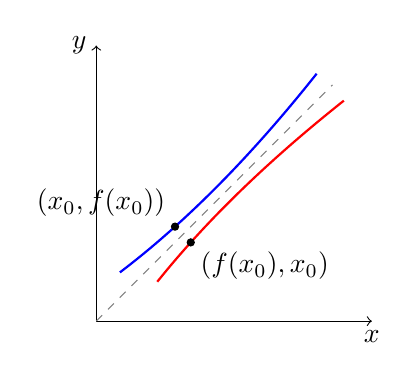
\begin{tikzpicture}[xscale=1.0]
	\draw[->] (0,0) -- (3.5,0) node[below] {$x$};
	\draw[->] (0,0) -- (0,3.5) node[left] {$y$};
	\draw[dashed,gray] (0,0)--(3,3);
	\draw[blue,thick,domain=0.3:2.8,samples=80] plot (\x,{0.4+0.7*\x+0.1*\x*\x});
	\draw[red,thick,domain=0.5:2.8,samples=80] plot ({0.4+0.7*\x+0.1*\x*\x},{\x});
	\fill (1,1.2) circle (1.5pt); \node[above left] at (1,1.2) {$(x_0, f(x_0))$};
	\fill (1.2,1) circle (1.5pt); \node[below right] at (1.2,1) {$(f(x_0), x_0)$};
	\end{tikzpicture}
	\caption{Inverse.}
	\label{fig:inverse}
\end{figure}

\subsection{Integration theorems}

\begin{proof}[Proof of Lemma~\ref{lem:barrow-area}]
	For $\mathrm{d}x>0$\comma $f(x_0)\le f\le f(x_0+\mathrm{d}x)$ on the interval; inscribed/circumscribed rectangles bound $A$. For $\mathrm{d}x<0$\comma use \eqref{eq:oriented-area}.\hfill$\square$
\end{proof}

\begin{figure}[H]
	\centering
	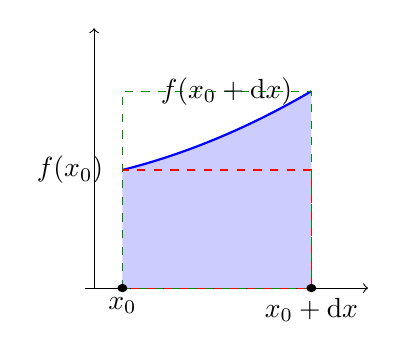
\begin{tikzpicture}[xscale=1.2,yscale=1.0]
	\draw[->] (2.6,0) -- (5.6,0); \draw[->] (2.7,0) -- (2.7,3.3);
	\fill[blue!20] (3,0) -- plot[domain=3:5,samples=60] (\x,{1.5+0.3*(\x-3)+0.1*(\x-3)*(\x-3)}) -- (5,0) -- cycle;
	\draw[blue,thick,domain=3:5,samples=60,smooth] plot (\x,{1.5+0.3*(\x-3)+0.1*(\x-3)*(\x-3)});
	\draw[dashed,red] (3,0) rectangle (5,1.5);
	\draw[dashed,green!55!black] (3,0) rectangle (5,2.5);
	\fill (3,0) circle (1.5pt); \node[below] at (3,0) {$x_0$};
	\fill (5,0) circle (1.5pt); \node[below] at (5,0) {$x_0+\mathrm{d}x$};
	\node[left] at (2.9,1.5) {$f(x_0)$};
	\node[left] at (4.9,2.5) {$f(x_0+\mathrm{d}x)$};
	\end{tikzpicture}
	\caption{Barrow's area inequality.}
	\label{fig:area-ineq}
\end{figure}

\begin{proof}[Proof of Lemma~\ref{lem:mvt-int}]
	$G(t)=A_{x_0}^t$ is differentiable with $G'=f$; MVT on the interval gives $\theta$ with $A_{x_0}^{x_0+\mathrm{d}x}=f(\theta)\mathrm{d}x$.\hfill$\square$
\end{proof}

\begin{proof}[Proof of Theorem~\ref{thm:fftc}]
	Fix $x_0\in(a\comma b)$ and $\varepsilon>0$. Let $h\ne0$ with $x_0+h\in[a\comma b]$\comma and let $I_h$ be the closed interval with endpoints $x_0$ and $x_0+h$. Since $f$ is continuous at $x_0$\comma for $|h|$ sufficiently small there are constants $m_\varepsilon\comma M_\varepsilon$ with $m_\varepsilon\le f(u)\le M_\varepsilon$ on $I_h$\comma $|m_\varepsilon-f(x_0)|<\varepsilon$\comma $|M_\varepsilon-f(x_0)|<\varepsilon$. By integral monotonicity applied on $I_h$ to the constant functions $m_\varepsilon$ and $M_\varepsilon$\comma for $h>0$ one has $m_\varepsilon h\le A_{x_0}^{x_0+h}\le M_\varepsilon h$; for $h<0$ the same inequality holds with both directions reversed (the oriented convention \eqref{eq:oriented-area} changes the sign of both $A_{x_0}^{x_0+h}$ and $h$). In either case\comma dividing by $h$ preserves the direction of the inequality (both sides change sign together with $h$)\comma giving
	\[
	m_\varepsilon\;\le\;\frac{A_a^{x_0+h}-A_a^{x_0}}{h}\;\le\;M_\varepsilon\comma
	\]
	where the numerator uses additivity \eqref{eq:lin-int}. Since $\varepsilon>0$ was arbitrary and $m_\varepsilon\comma M_\varepsilon\to f(x_0)$ as $\varepsilon\to0$\comma the squeeze yields $\frac{d}{dx}A_a^x|_{x_0}=f(x_0)$; since $x_0\in(a\comma b)$ was arbitrary\comma \eqref{eq:fftc} holds on $(a\comma b)$\comma and the one-sided cases at $x=a\comma b$ follow by one-sided limits.\hfill$\square$
\end{proof}

\begin{figure}[H]
	\centering
	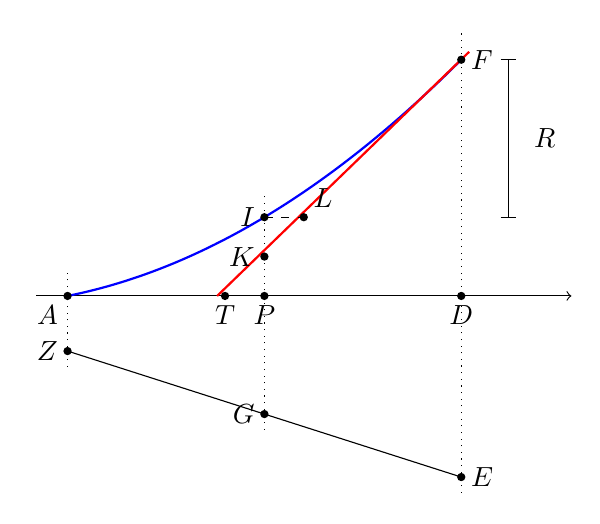
\begin{tikzpicture}[xscale=1.0]
	\draw[->] (-0.4,0) -- (6.4,0);
	\draw[dotted] (0,-0.9) -- (0,0.3);
	\draw[dotted] (2.5,-1.7) -- (2.5,1.3);
	\draw[dotted] (5,-2.5) -- (5,3.4);
	\draw plot[smooth,tension=0.7] coordinates {(0,-0.7) (2.5,-1.5) (5,-2.3)};
	\draw[blue,thick,domain=0:5,samples=100,smooth] plot (\x,{0.08*\x*\x+0.2*\x});
	\draw[red,thick] (1.9,0)--(5.1,3.1);
	\draw[dashed] (2.5,1) -- (3,1);
	\fill (0,0) circle (1.5pt);    \node[below left]  at (0,0)    {$A$};
	\fill (2,0) circle (1.5pt);    \node[below]       at (2,0)    {$T$};
	\fill (2.5,0) circle (1.5pt);  \node[below]       at (2.5,0)  {$P$};
	\fill (5,0) circle (1.5pt);    \node[below]       at (5,0)    {$D$};
	\fill (0,-0.7) circle (1.5pt); \node[left]        at (0,-0.7) {$Z$};
	\fill (2.5,-1.5) circle (1.5pt);\node[left]       at (2.5,-1.5){$G$};
	\fill (5,-2.3) circle (1.5pt); \node[right]       at (5,-2.3) {$E$};
	\fill (2.5,1) circle (1.5pt);  \node[left]        at (2.5,1)  {$I$};
	\fill (2.5,0.5) circle (1.5pt);\node[left]        at (2.5,0.5){$K$};
	\fill (3,1) circle (1.5pt);    \node[above right] at (3,1)    {$L$};
	\fill (5,3) circle (1.5pt);    \node[right]       at (5,3)    {$F$};
	\draw (5.5,1) -- (5.7,1); \draw (5.5,3) -- (5.7,3); \draw (5.6,1) -- (5.6,3);
	\node[right] at (5.8,2) {$R$};
	\end{tikzpicture}
	\caption{Barrow's Fig.~109.}
	\label{fig:barrow109}
\end{figure}

\begin{proof}[Proof of Theorem~\ref{thm:second-ftc}]
	$G(x)=\int_a^x f$ has $G'=f$; so $(F-G)'=0$ and $F-G$ is constant; $F(b)-F(a)=\int_a^b f$.\hfill$\square$
\end{proof}

\begin{figure}[H]
	\centering
	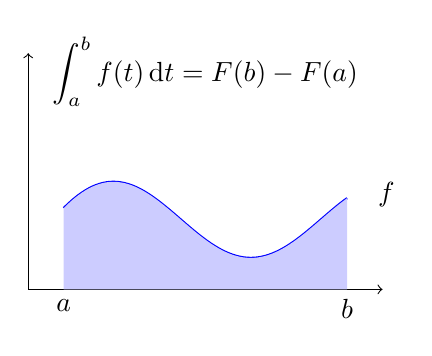
\begin{tikzpicture}[xscale=0.9]
	\draw[->] (0,0) -- (5,0); \draw[->] (0,0) -- (0,3);
	\draw[blue,thick,domain=0.5:4.5,samples=80] plot (\x,{0.5+0.6*sin(\x*1.5 r)+0.5*sin(\x*0.5 r)});
	\fill[blue!20] (0.5,0) -- plot[domain=0.5:4.5,samples=80] (\x,{0.5+0.6*sin(\x*1.5 r)+0.5*sin(\x*0.5 r)}) -- (4.5,0) -- cycle;
	\node[above] at (2.5,2.2) {$\displaystyle \int_a^b f(t)\,\mathrm{d}t = F(b)-F(a)$};
	\node[below] at (0.5,0) {$a$}; \node[below] at (4.5,0) {$b$};
	\node[right] at (4.8,1.2) {$f$};
	\end{tikzpicture}
	\caption{Second FTC.}
	\label{fig:second-ftc}
\end{figure}

\begin{proof}[Proof of Theorem~\ref{thm:ibp}]
	$(fg)'=f'g+fg'$; integrate with Second FTC.\hfill$\square$
\end{proof}

\begin{proof}[Proof of Theorem~\ref{thm:subst}]
	Let $F'=f$. Chain rule: $(F\circ g)'=f(g)g'$; Second FTC on both sides yields \eqref{eq:subst}.\hfill$\square$
\end{proof}

\begin{proof}[Proof of Theorem~\ref{thm:weighted-mvt}]
	$m\le f\le M$ and $w\ge0$ give $m\int w\le\int fw\le M\int w$; so $A:=\int fw/\int w\in[m\comma M]$; by IVT $f(c)=A$.\hfill$\square$
\end{proof}

\subsection{The logarithm and the exponential}

\begin{proof}[Proof of Theorem~\ref{thm:log}]
	$\ln(ab)-\ln(b)=\int_b^{ab}\mathrm{d}t/t$; the map $(t\comma y)\mapsto(t/b\comma by)$ preserves area and preserves $y=1/t$\comma so this equals $\int_1^a\mathrm{d}u/u=\ln a$.\hfill$\square$
\end{proof}

\begin{figure}[H]
	\centering
	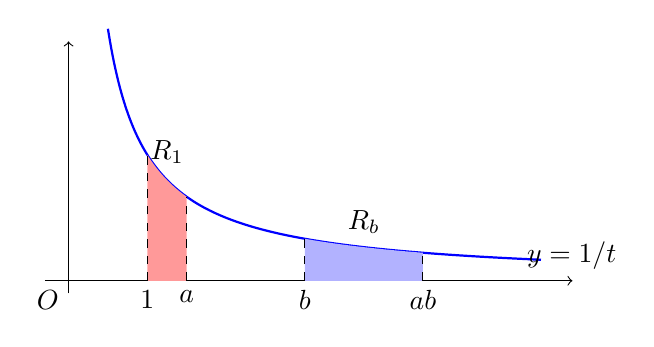
\begin{tikzpicture}[xscale=1.0,yscale=1.6]
	\draw[->] (-0.3,0) -- (6.4,0); \draw[->] (0,-0.1) -- (0,1.9);
	\draw[blue,thick,domain=0.5:6,samples=150,smooth] plot (\x,{1/\x});
	\fill[red!40] (1,0) -- plot[domain=1:1.5,samples=30] (\x,{1/\x}) -- (1.5,0) -- cycle;
	\fill[blue!30] (3,0) -- plot[domain=3:4.5,samples=30] (\x,{1/\x}) -- (4.5,0) -- cycle;
	\draw[dashed] (1,0) -- (1,1); \draw[dashed] (1.5,0) -- (1.5,0.667);
	\draw[dashed] (3,0) -- (3,0.333); \draw[dashed] (4.5,0) -- (4.5,0.222);
	\node[below] at (1,0) {$1$}; \node[below] at (1.5,0) {$a$};
	\node[below] at (3,0) {$b$}; \node[below] at (4.5,0) {$ab$};
	\node[above] at (1.25,0.85) {$R_1$};
	\node[above] at (3.75,0.30) {$R_b$};
	\node[right] at (5.7,0.20) {$y=1/t$};
	\node[below left] at (0,0) {$O$};
	\end{tikzpicture}
	\caption{Hyperbolic similarity.}
	\label{fig:hyperbola}
\end{figure}

\begin{proof}[Proof of Theorem~\ref{thm:exp}]
	$\ln(\exp u\exp v)=\ln(\exp u)+\ln(\exp v)=u+v=\ln(\exp(u+v))$; injectivity of $\ln$ gives \eqref{eq:exp}.\hfill$\square$
\end{proof}

\begin{proof}[Proof of Theorem~\ref{thm:image}]
	Sign-Law gives $\exp(\R_{<0})={]}0\comma1[$\comma $\exp(\{0\})=\{1\}$\comma $\exp(\R_{>0})={]}1\comma\infty[$; Image-Union gives $\exp(\R)=\R_{>0}$. Bijectivity gives $\ln(\R_{>0})=\R$.\hfill$\square$
\end{proof}

\begin{figure}[H]
	\centering
	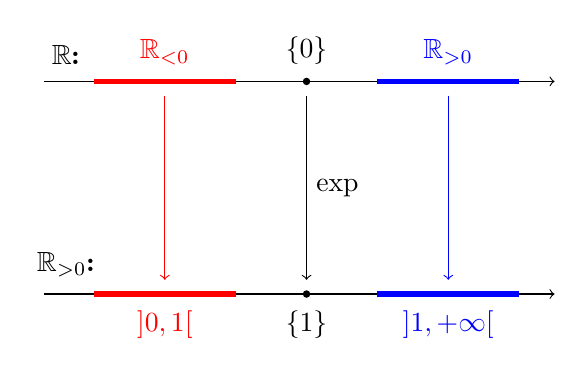
\begin{tikzpicture}[xscale=0.9,yscale=0.9]
	\draw[->] (-0.2,0) -- (7,0);
	\node[above] at (0.1,0.1) {$\R$:};
	\draw[red,line width=2pt] (0.5,0)--(2.5,0);
	\node[above] at (1.5,0.1) {\textcolor{red}{$\R_{<0}$}};
	\fill (3.5,0) circle (1.5pt);
	\node[above] at (3.5,0.1) {$\{0\}$};
	\draw[blue,line width=2pt] (4.5,0)--(6.5,0);
	\node[above] at (5.5,0.1) {\textcolor{blue}{$\R_{>0}$}};
	\draw[->,red]  (1.5,-0.2) -- (1.5,-2.8);
	\draw[->]      (3.5,-0.2) -- (3.5,-2.8);
	\draw[->,blue] (5.5,-0.2) -- (5.5,-2.8);
	\node[right] at (3.5,-1.5) {$\exp$};
	\draw[->] (-0.2,-3) -- (7,-3);
	\node[above] at (0.1,-2.9) {$\R_{>0}$:};
	\draw[red,line width=2pt] (0.5,-3)--(2.5,-3);
	\node[below] at (1.5,-3.1) {\textcolor{red}{${]}0,1[$}};
	\fill (3.5,-3) circle (1.5pt);
	\node[below] at (3.5,-3.1) {$\{1\}$};
	\draw[blue,line width=2pt] (4.5,-3)--(6.5,-3);
	\node[below] at (5.5,-3.1) {\textcolor{blue}{${]}1,+\infty[$}};
	\end{tikzpicture}
	\caption{Image of Exponential Function $\exp$}
	\label{fig:exp-image}
\end{figure}

\section{Remarks on the geometric development}

Barrow's sliding-tangent MVT proof is retained for its historical content; the Barrow-tangency principle \eqref{eq:barrow-tangency} is eliminable via Rolle and Monotone + MVT. The FFTC proof uses only area additivity \eqref{eq:lin-int} and rectangle comparison \eqref{eq:barrow-area}; no Riemann-sum limit is invoked\comma as emphasized by Barrow \cite{Barrow1916} and confirmed in Part~II.

\subsection*{Dependency summary}

EVT\comma IVT $\to$ Fermat $\to$ Rolle $\to$ MVT $\to$ Const\comma Monotone\comma Cauchy\comma Darboux\comma Taylor\comma Convexity\comma Inverse. Second FTC from FFTC + Const. IBP\comma Subst\comma Weighted MVT from Second FTC or IVT/IntMono. Log from IntAdd + Similarity; Exp from Log; Image from LnBij + Sign-Law + ImgUnion. Barrow-area + MVTInt $\to$ FFTC $\to$ Log.

\part{Reverse-Mathematical Analysis in $\mathsf{RCA}_0$}

\noindent Every Part~I entry reappears as a tagged statement with a dependency table and an exact strength in $\{\textsf{FOL}\comma\textsf{RCA}_0\comma\textsf{WKL}_0\comma\textsf{ACA}_0\comma\textsf{ZF}\comma\textsf{ZFC}\}$. Geometric proofs are at most $\textsf{WKL}_0$ as written; \S\ref{sec:core-proofs} gives the matching $\textsf{RCA}_0$-strength tables via Hardin--Velleman\comma Yokoyama\comma or direct argument.

\section{Coding conventions}
\label{sec:coding}

\noindent Following Yokoyama \cite{Yokoyama2010}\comma we distinguish:
\begin{itemize}
	\item \emph{Pointwise differentiability:} the limit exists for each $x\in I$; no derivative function needed. Hardin--Velleman's Rolle and MVT in $\textsf{RCA}_0$ use this.
	\item \emph{Strong $C^k$-coding:} $C^k_{\mathrm{strong}}(I)(f):\iff\exists g_0\comma\dots\comma g_k:\ g_0=f\wedge\forall j<k\comma\ g_{j+1}=g_j'$. All $C^k$ hypotheses in Part~II mean strong $C^k$-coding.
	\item \emph{Inverse function:} Yokoyama \cite[Thm.~3.22]{Yokoyama2010} in $\textsf{RCA}_0$ for strong $C^1$-functions with $f'\ne0$ on $I$\comma $x_0\in I^\circ$. The pointwise form is not $\textsf{RCA}_0$-provable.
\end{itemize}

\section{Research context}\label{sec:research}
\subsection{The core hierarchy}
$\textsf{RCA}_0$ = recursive comprehension + $\Sigma^0_1$-induction; no choice.
\begin{center}\small
	\noindent\begin{tabular}{|>{\raggedright\arraybackslash}m{4.5cm}|>{\centering\arraybackslash}m{2.2cm}|>{\centering\arraybackslash}m{3.2cm}|>{\centering\arraybackslash}m{1.3cm}|}
		\hline
		\textbf{Result} & \textbf{Strength} & \textbf{Reference} & \textbf{Choice} \\ \hline
		\textsf{MVT} & \textsf{RCA$_0$} & \cite{HardinVelleman2001} & \textsf{none} \\ \hline
		\textsf{IVT}\comma \textsf{EVT} & \textsf{WKL$_0$} & \cite{Simpson2009} & \textsf{none} \\ \hline
		\textsf{sequential IVT/MVT} & $\equiv\textsf{WKL}_0$ & \cite{Simpson2009,Sanders2020} & \textsf{none} \\ \hline
		$\ln$/$\exp$ chain & \textsf{RCA$_0$} & \cite{Yokoyama2010} & \textsf{none} \\ \hline
	\end{tabular}
\end{center}

\noindent Key facts:
\begin{itemize}
	\item \textbf{MVT $\in\textsf{RCA}_0$} (Hardin--Velleman \cite{HardinVelleman2001}); no EVT\comma no IVT.
	\item \textbf{IVT $\equiv\textsf{WKL}_0$}: sole non-$\textsf{RCA}_0$ ingredient is $\sup\{x:f(x)<0\}$.
	\item \textbf{Inverse function $\in\textsf{RCA}_0$} (Yokoyama \cite[Thm.~3.22]{Yokoyama2010}).
	\item \textbf{$\ln$/$\exp$ $\in\textsf{RCA}_0$}: definitional plus integral postulates.
\end{itemize}

\setcounter{theorem}{0}
\begin{remark}[Proofs vs.\ classification]
Part~I proofs use $\sup$\comma $\inf$\comma LUB (\textsf{ax:R-complete}). MVT is $\textsf{RCA}_0$ via Hardin--Velleman. IVT\comma EVT are $\textsf{WKL}_0$-equivalent over $\textsf{RCA}_0$ and remain $\textsf{WKL}_0$.
\end{remark}

\subsection{Illustrative theorems}

\bigskip
\begin{center}\small
	\begin{tabular}{|>{\raggedright\arraybackslash}m{4.5cm}|>{\centering\arraybackslash}m{2.5cm}|>{\centering\arraybackslash}m{3.2cm}|>{\centering\arraybackslash}m{1.3cm}|}
		\hline
		\textbf{Theorem} & \textbf{Strength} & \textbf{Reference} & \textbf{Choice} \\ \hline
		\textsf{IVT} & \textsf{WKL$_0$} & \cite{Simpson2009} & \textsf{none} \\ \hline
		\textsf{MVT} & \textsf{RCA$_0$} & \cite{HardinVelleman2001} & \textsf{none} \\ \hline
		\textsf{Hahn--Banach} & $\equiv\textsf{WKL}_0$ & \cite{Simpson2009} & \textsf{none} \\ \hline
		\textsf{Weierstrass approx.} & $\equiv\textsf{WKL}_0$ & \cite{Simpson2009} & \textsf{none} \\ \hline
		\textsf{Peano existence} & $\equiv\textsf{WKL}_0$ & \cite{Simpson2009} & \textsf{none} \\ \hline
		\textsf{sequential IVT/MVT} & $\equiv\textsf{WKL}_0$ & \cite{Sanders2020} & \textsf{none} \\ \hline
		\textsf{separation} & $\equiv\textsf{ACA}_0$ & \cite{Humphreys2015} & \textsf{none} \\ \hline
		\textsf{Banach--Alaoglu} & \textsf{ZFC} & \cite{Alaoglu1940} & \textsf{full AC} \\ \hline
		\textsf{Tychonoff} & \textsf{ZFC} & \cite{Kelley1950} & \textsf{full AC} \\ \hline
		\textsf{well-ordering} & \textsf{ZFC} & \cite{Jech1973} & \textsf{full AC} \\ \hline
	\end{tabular}
\end{center}

\noindent Strictness: $\textsf{RCA}_0\subsetneq\textsf{WKL}_0\subsetneq\textsf{ACA}_0\subsetneq\textsf{ZFC}$.

\subsection{Dedekind vs.\ Cauchy completeness}

\begin{itemize}
	\item \textbf{Dedekind (LUB):} every nonempty bounded-above subset has a supremum. A $\textsf{ZF}$ theorem; equivalent over ordered fields to IVT\comma EVT\comma MVT\comma Darboux \cite{Propp2012,Teismann2013}. Form used here: \textsf{ax:R-complete}.
	\item \textbf{Cauchy completeness:} every Cauchy sequence converges. $\textsf{ZF}$-equivalent to $\textsf{DC}_\R$. Not a $\textsf{ZF}$ theorem. Not used here.
\end{itemize}

Solovay's model \cite{Solovay1970}: under $\textsf{ZF}+\textsf{DC}$\comma all reals are Lebesgue measurable and $\textsf{AC}$ fails; $\textsf{DC}\Rightarrow\textsf{DC}_\R$\comma so Cauchy completeness holds there. The choice-free classification is strictly finer than $\textsf{DC}_\R$.

\subsection{Constructive RM}

In BISH\comma IVT $\equiv\textsf{LLPO}$ \cite{Bridges2023}. This document is classical.

\subsection{Lean~4 and Mathlib}

Lean~4 and Mathlib \cite{Lean4}: about $70.4\%$ of declarations depend on \textsf{Classical.choice}\comma and $13.1\%$ have choice-free statements with choice-dependent proofs \cite{Crossref2026}. Our classification is stronger: it certifies choice-free proofs\comma not just statements.

\section{Axioms}
\label{sec:axioms}

\noindent The fourteen axioms of $\R$ as a complete ordered field.

\medskip

\noindent$\begin{array}{|C|L|R|C|}
\hline
\swpax{ax:R-add-assoc}{axi:R-add-assoc} &
\textsf{ax{:}add{-}assoc}:\forall (x\comma y\comma z:\R)\comma\;(x+y)+z=x+(y+z) &
\textsf{Add.}\allowbreak\textsf{Assoc.} & $\textsf{ZF}$ \\ \hline
\swpax{ax:R-add-comm}{axi:R-add-comm} &
\textsf{ax{:}add{-}comm}:\forall (x\comma y:\R)\comma\;x+y=y+x &
\textsf{Add.}\allowbreak\textsf{Comm.} & $\textsf{ZF}$ \\ \hline
\end{array}$
\par\nointerlineskip\noindent$\begin{array}{|C|L|R|C|}
\hline
\swpax{ax:R-add-zero}{axi:R-add-zero} &
\textsf{ax{:}add{-}zero}:\forall (x:\R)\comma\;0+x=x &
\textsf{Add.}\allowbreak\textsf{Id.} & $\textsf{ZF}$ \\ \hline
\swpax{ax:R-add-inv}{axi:R-add-inv} &
\textsf{ax{:}add{-}inv}:\forall (x:\R)\comma\;x+(-x)=0 &
\textsf{Add.}\allowbreak\textsf{Inv.} & $\textsf{ZF}$ \\ \hline
\end{array}$
\par\nointerlineskip\noindent$\begin{array}{|C|L|R|C|}
\hline
\swpax{ax:R-mul-assoc}{axi:R-mul-assoc} &
\textsf{ax{:}mul{-}assoc}:\forall (x\comma y\comma z:\R)\comma\;(x\cdot y)\cdot z=x\cdot(y\cdot z) &
\textsf{Mul.}\allowbreak\textsf{Assoc.} & $\textsf{ZF}$ \\ \hline
\swpax{ax:R-mul-comm}{axi:R-mul-comm} &
\textsf{ax{:}mul{-}comm}:\forall (x\comma y:\R)\comma\;x\cdot y=y\cdot x &
\textsf{Mul.}\allowbreak\textsf{Comm.} & $\textsf{ZF}$ \\ \hline
\end{array}$
\par\nointerlineskip\noindent$\begin{array}{|C|L|R|C|}
\hline
\swpax{ax:R-mul-one}{axi:R-mul-one} &
\textsf{ax{:}mul{-}one}:\forall (x:\R)\comma\;1\cdot x=x &
\textsf{Mul.}\allowbreak\textsf{Id.} & $\textsf{ZF}$ \\ \hline
\swpax{ax:R-mul-inv}{axi:R-mul-inv} &
\textsf{ax{:}mul{-}inv}:\forall (x:\R)\comma\;(x\ne0\to x\cdot x^{-1}=1)\wedge(x=0\to x^{-1}=0) &
\textsf{Mul.}\allowbreak\textsf{Inv.} & $\textsf{ZF}$ \\ \hline
\end{array}$
\par\nointerlineskip\noindent$\begin{array}{|C|L|R|C|}
\hline
\swpax{ax:R-distrib}{axi:R-distrib} &
\textsf{ax{:}distrib}:\forall (x\comma y\comma z:\R)\comma\;x\cdot(y+z)=x\cdot y+x\cdot z &
\textsf{Distrib.} & $\textsf{ZF}$ \\ \hline
\swpax{ax:R-nontriv}{axi:R-nontriv} &
\textsf{ax{:}nontriv}:0\ne1 &
\textsf{Nontriv.} & $\textsf{ZF}$ \\ \hline
\end{array}$
\par\nointerlineskip\noindent$\begin{array}{|C|L|R|C|}
\hline
\swpax{ax:R-order}{axi:R-order} &
\textsf{ax{:}order}:\bigl(\forall x:\,x\le x\bigr)\wedge\bigl(\forall x\comma y:\,x\le y\wedge y\le x\to x=y\bigr)\wedge\bigl(\forall x\comma y\comma z:\,x\le y\wedge y\le z\to x\le z\bigr)\wedge\bigl(\forall x\comma y:\,x\le y\vee y\le x\bigr) &
\textsf{Linear}\allowbreak\textsf{Order} & $\textsf{ZF}$ \\ \hline
\swpax{ax:R-add-monotone}{axi:R-add-monotone} &
\textsf{ax{:}add{-}mon}:\forall (x\comma y\comma z:\R)\comma\;x\le y\to x+z\le y+z &
\textsf{Add}\allowbreak\textsf{Mon.} & $\textsf{ZF}$ \\ \hline
\end{array}$
\par\nointerlineskip\noindent$\begin{array}{|C|L|R|C|}
\hline
\swpax{ax:R-mul-monotone-pos}{axi:R-mul-monotone-pos} &
\textsf{ax{:}mul{-}mon}:\forall (x\comma y:\R)\comma\;0\le x\wedge0\le y\to0\le x\cdot y &
\textsf{Mul}\allowbreak\textsf{Mon.} & $\textsf{ZF}$ \\ \hline
\swpax{ax:R-complete}{axi:R-complete} &
\textsf{ax{:}complete}:\bigl(\exists x\comma S(x)\bigr)\wedge\bigl(\exists u\comma\forall x\comma S(x)\to x\le u\bigr)\to\exists s\comma\bigl(\forall x\comma S(x)\to x\le s\bigr)\wedge\bigl(\forall u\comma(\forall x\comma S(x)\to x\le u)\to s\le u\bigr) &
\textsf{Cut} & $\textsf{ZF}$ \\ \hline
\end{array}$

\medskip

\noindent The Cut axiom enters no Part~II proof; it is $\textsf{ZF}$-realizable via Dedekind cuts without choice.

\section{Postulates}
\label{sec:postulates}

\noindent Unproved internal statements. Each is $\textsf{RCA}_0$-provable or first-order logical; none introduces choice.

\subsection{Integral postulates}
\noindent$\begin{array}{|C|L|R|C|}
\hline
\swppos{pos:int-linear}{posi:int-linear} &
\textsf{Pos{:}IntLinear}:\forall (a,b:\R),\;\forall (f,g\in L^{1}([a,b])),\;\forall (\alpha,\beta:\R),\;\int_{a}^{b}(\alpha f(x)+\beta g(x))\,dx=\alpha\int_{a}^{b}f(x)\,dx+\beta\int_{a}^{b}g(x)\,dx &
\textsf{IntLin} & $\textsf{RCA}_0$ \\ \hline
\swppos{pos:int-add}{posi:int-add} &
\textsf{Pos{:}IntAdd}:\forall (a,b,c:\R),\;\forall (f\in L^{1}([\min(a,b,c),\max(a,b,c)])),\;\int_{a}^{b}f(x)\,dx=\int_{a}^{c}f(x)\,dx+\int_{c}^{b}f(x)\,dx &
\textsf{IntAdd} & $\textsf{RCA}_0$ \\ \hline
\end{array}$
\par\noindent{\footnotesize\textsf{Note:} \(f\in L^1([\alpha,\beta])\) and \([\gamma,\delta]\subseteq[\alpha,\beta]\) imply \(f\in L^1([\gamma,\delta])\); cited as \texttt{restrict} in proof tables.}
\par\nointerlineskip\noindent$\begin{array}{|C|L|R|C|}
\hline
\swppos{pos:int-mono}{posi:int-mono} &
\textsf{Pos{:}IntMono}:\forall (a,b:\R),\;a<b\to\forall (f,g\in L^{1}([a,b])),\;\bigl(\forall (x\in[a,b]),\;f(x)\le g(x)\bigr)\to\int_{a}^{b}f(x)\,dx\le\int_{a}^{b}g(x)\,dx &
\textsf{IntMono} & $\textsf{RCA}_0$ \\ \hline
\swppos{pos:int-subst}{posi:int-subst} &
\textsf{Pos{:}IntSubst}:\forall (a,b:\R),\;\forall (g:\R\to\R),\;\forall (f:\R\to\R),\;
g\in C^{1}([\min(a,b),\max(a,b)])\wedge
\bigl(\forall t\in[\min(a,b),\max(a,b)],\;g^{\prime}(t)\neq0\bigr)\wedge
f\in C^{0}(g([\min(a,b),\max(a,b)]))
\to\int_{g(a)}^{g(b)}f(x)\,dx=\int_{a}^{b}f(g(t))\,g^{\prime}(t)\,dt &
\textsf{IntSubst} & $\textsf{RCA}_0$ \\ \hline
\end{array}$
\par\nointerlineskip\noindent$\begin{array}{|C|L|R|C|}
\hline
\swppos{pos:int-cont-integ}{posi:int-cont-integ} &
\textsf{Pos{:}ContInt}:\forall (a,b:\R),\;a<b\to\forall (f:\R\to\R),\;f\in C^{0}([a,b])\to f\in L^{1}([a,b]) &
\textsf{ContInt} & $\textsf{RCA}_0$ \\ \hline
\swppos{pos:similarity}{posi:similarity} &
\textsf{Pos{:}Similarity}:\forall (a,b:\R),\;0<a\wedge0<b\to\forall (h:\R\to\R),\;\int_{b}^{a\cdot b}h(t)\,dt=\int_{1}^{a}h(bu)\cdot b\,du&
\textsf{Sim.} & $\textsf{RCA}_0$ \\ \hline
\end{array}$

\subsection{Differential postulates}
\noindent$\begin{array}{|C|L|R|C|}
\hline
\swppos{pos:prod-rule}{posi:prod-rule} &
\textsf{Pos{:}ProdRule}:\forall (f,g:\R\to\R),\;\forall (x:\R),\;\mathsf{Diff}(f,x)\wedge\mathsf{Diff}(g,x)\to\mathsf{Diff}(f\cdot g,x)\wedge(f\cdot g)^{\prime}(x)=f^{\prime}(x)g(x)+f(x)g^{\prime}(x) &
\textsf{Prod} & $\textsf{RCA}_0$ \\ \hline
\swppos{pos:chain-rule}{posi:chain-rule} &
\textsf{Pos{:}ChainRule}:\forall (f,g:\R\to\R),\;\forall (x:\R),\;\mathsf{Diff}(g,x)\wedge\mathsf{Diff}(f,g(x))\to\mathsf{Diff}(f\circ g,x)\wedge(f\circ g)^{\prime}(x)=f^{\prime}(g(x))\cdot g^{\prime}(x) &
\textsf{Chain} & $\textsf{RCA}_0$ \\ \hline
\end{array}$
\par\nointerlineskip\noindent$\begin{array}{|C|L|R|C|}
\hline
\swppos{pos:inv-cont}{posi:inv-cont} &
\textsf{Pos{:}InvCont}:\bigl(t\mapsto1/t\bigr)\in C^{0}(\R_{>0}) &
\textsf{InvCont} & $\textsf{RCA}_0$ \\ \hline
\swppos{pos:barrow-tangency}{posi:barrow-tangency} &
\textsf{Pos{:}BarrowTangency}:\forall (G:\R\to\R),\;\forall (x_0,m:\R),\;\mathsf{Diff}(G,x_0)\wedge
\Bigl(\bigl(\forall (u\neq x_0)\ \text{near}\ x_0,\;G(x_0)+m(u-x_0)\le G(u)\bigr)\vee
\bigl(\forall (u\neq x_0)\ \text{near}\ x_0,\;G(x_0)+m(u-x_0)\ge G(u)\bigr)\Bigr)\to m=G^{\prime}(x_0) &
\textsf{Barrow} & $\textsf{RCA}_0$ \\ \hline
\end{array}$

\subsection{Logarithmic postulates}
\noindent$\begin{array}{|C|L|R|C|}
\hline
\swppos{pos:ln-bij}{posi:ln-bij} &
\textsf{Pos{:}LnBij}:\mathsf{Bijective}(\ln:\R_{>0}\to\R) &
\textsf{LnBij} & $\textsf{RCA}_0$ \\ \hline
\swppos{pos:ln-sign}{posi:ln-sign} &
\textsf{Pos{:}LnSign}:\forall (a:\R_{>0}),\;
\bigl(\ln(a)<0\leftrightarrow a<1\bigr)\wedge
\bigl(\ln(a)=0\leftrightarrow a=1\bigr)\wedge
\bigl(\ln(a)>0\leftrightarrow a>1\bigr) &
\textsf{LnSign} & $\textsf{RCA}_0$ \\ \hline
\end{array}$

\subsection{Logical postulate}
\noindent$\begin{array}{|C|L|R|C|}
\hline
\swppos{pos:img-union}{posi:img-union} &
\textsf{Pos{:}ImgUnion}:\forall (X,Y:\mathsf{Type}),\;\forall (f:X\to Y),\;\forall (A,B:X\to\mathsf{Prop}),\;
f(A\cup B)=f(A)\cup f(B) &
\textsf{ImgUnion} & $\textsf{FOL}$ \\ \hline
\end{array}$

\subsection{External results}
\noindent$\begin{array}{|C|L|R|C|}
\hline
\swppos{pos:cont-img-bdd}{posi:cont-img-bdd} &
\textsf{Pos{:}ContImgBdd}:\forall (f:[a,b]\to\R),\ f\in C^{0}([a,b])\to
\bigl(\exists L,U:\R,\ \forall x:[a,b],\ L\le f(x)\le U\bigr) &
\textsf{BddImg} & $\textsf{RCA}_0$ \\ \hline
\swppos{pos:cont-img-attain}{posi:cont-img-attain} &
\textsf{Pos{:}ContImgAttain}:\forall (f:[a,b]\to\R),\ f\in C^{0}([a,b])\to
\bigl(\exists x_{\max}:[a,b],\forall x:[a,b],f(x)\le f(x_{\max})\bigr)
\wedge\bigl(\exists x_{\min}:[a,b],\forall x:[a,b],f(x_{\min})\le f(x)\bigr) &
\textsf{Attain} & $\textsf{WKL}_0$ \\ \hline
\end{array}$

\text{\  }\medskip

\noindent{\footnotesize\textsf{Note on \textsf{Pos:ContImgBdd} and the coding of $C^0([a,b])$.} Under the coding of \S\ref{sec:coding} (following Simpson \cite{Simpson2009}), a continuous function $f:[a,b]\to\R$ carries a coded modulus of continuity, from which boundedness of the image $f([a,b])$ follows in $\textsf{RCA}_0$. The \textsf{Pos:ContImgBdd} tag $\textsf{RCA}_0$ reflects this standard coding convention. Under an alternative coding --- pointwise continuity without a coded modulus --- boundedness of continuous functions on $[a,b]$ rises to $\textsf{WKL}_0$; the choice between codings is a foundation choice, not a mathematical error, and \S\ref{sec:coding} fixes the Simpson convention for this document.}
\medskip
\par\nointerlineskip\noindent$\begin{array}{|C|L|R|C|}
\hline
\swppos{pos:pi01-sup}{posi:pi01-sup} &
\textsf{Pos{:}}\Pi^{0}_{1}\textsf{Sup}:\forall (\varphi:\N\times\R\to\{0,1\}),\;\forall (a,b:\R),\;a\le b\to
\bigl(\exists x\in[a,b],\forall n\,\varphi(n,x)=0\bigr)\to
\exists s\in[a,b],\;
\bigl(\forall x\in[a,b],(\forall n\,\varphi(n,x)=0)\to x\le s\bigr)\wedge
\bigl(\forall u\in[a,b],(\forall x\in[a,b],(\forall n\,\varphi(n,x)=0)\to x\le u)\to s\le u\bigr) &
\textsf{Sup} & $\textsf{WKL}_0$ \\ \hline
\swppos{pos:sigma01-choice}{posi:sigma01-choice} &
\textsf{Pos{:}}\Sigma^{0}_{1}\textsf{Choice}:\bigl(\forall n,\exists m,R(n,m)\bigr)\to\exists g,\forall n,R(n,g(n)) &
\Sigma^0_1 & 
$\textsf{RCA}_0$ \\ \hline
\end{array}$
\par\nointerlineskip\noindent$\begin{array}{|C|L|R|C|}
\hline
\swppos{pos:seq-cont}{posi:seq-cont} &
\textsf{Pos{:}SeqCont}:\forall (f:[a,b]\to\R),f\in C^{0}([a,b])\to
\forall x:[a,b],\ \forall (x_n:\N\to[a,b]),\ (x_n\to x)\to \bigl(f(x_n)\to f(x)\bigr) &
\textsf{SeqCont} & $\textsf{RCA}_0$ \\ \hline
\swppos{pos:hv-rolle}{posi:hv-rolle} &
\textsf{Pos{:}HVRolle}:\forall (f:[a,b]\to\R),\;
f\in C^{0}([a,b])\wedge
\bigl(\forall x:(a,b),\ \mathsf{Diff}(f,x)\bigr)\wedge f(a)=f(b)\to
\exists c:(a,b),\ f^{\prime}(c)=0 &
\textsf{HVRolle} & $\textsf{RCA}_0$ \\ \hline
\end{array}$
\par\nointerlineskip\noindent$\begin{array}{|C|L|R|C|}
\hline
\swppos{pos:yokoyama-inv}{posi:yokoyama-inv} &
\textsf{Pos{:}YokoyamaInv}:\forall (f:I\to\R),\ \forall (x_0:I^{\circ}),\
C^{1}_{\mathrm{strong}}(I)(f)\wedge(\forall x:I,f^{\prime}(x)\neq 0)\wedge\mathsf{StrictMono}(f)\to
\mathsf{Diff}(f^{-1},f(x_0))\wedge(f^{-1})^{\prime}(f(x_0))=1/f^{\prime}(x_0) &
\textsf{YokInv} & $\textsf{RCA}_0$ \\ \hline
\end{array}$

\section{Definitions}
\label{sec:definitions}

\noindent Definitional abbreviations available in $\textsf{RCA}_0$: set notation by $\Delta^0_1$-comprehension; $L^1\comma C^k\comma C^k_{\mathrm{strong}}$ by $\Sigma^0_1$ predicates; $A_a^x\comma\ln\comma\exp$ by unique existence + graphs; \textsf{Diff}\comma\allowbreak \textsf{ChordSlope}\comma\allowbreak\textsf{TangentSlope}\comma\allowbreak\textsf{LocalExt}\comma\allowbreak\textsf{Increasing}\comma\textsf{StrictInc}\comma\allowbreak\textsf{StrictDec}\comma\allowbreak\textsf{StrictMono} by definitional extension.

\text{ \ }\\ 
\medskip
\noindent
\noindent$\begin{array}{|C|L|R|C|}
\hline
\swpdef{def:R-pos}{defi:R-pos} &
\mathsf{Def{:}R_{>0}}:\R_{>0}:=\{x:\R\mid x>0\},\;\R_{<0}:=\{x:\R\mid x<0\},\;\R_{\geq0}:=\{x:\R\mid x\geq0\} &
\textsf{R}_{\textsf{>0}} & $\textsf{RCA}_0$ \\ \hline
\swpdef{def:L1}{defi:L1} &
\mathsf{Def{:}L^{1}}:L^{1}([a,b]):=\{f:\R\to\R\mid\int_{a}^{b}|f(x)|\,dx<\infty\} &
\textsf{L}^{\textsf{1}} & $\textsf{RCA}_0$ \\ \hline
\end{array}$
\par\nointerlineskip\noindent$\begin{array}{|C|L|R|C|}
\hline
\swpdef{def:Ck}{defi:Ck} &
\mathsf{Def{:}C^{k}}:\forall (k:\N),\;\forall (U:\R\to\mathsf{Prop}),\;C^{k}(U):=\{f:\R\to\R\mid f\;\textsf{k}{-}\mathsf{times}\allowbreak \mathsf{cont.\ diff.\ on}\;U\} &
\textsf{C}^{\textsf{k}} & $\textsf{RCA}_0$ \\ \hline
\swpdef{def:strong-Ck}{defi:strong-Ck} &
\mathsf{Def{:}C^{k}_{\mathrm{strong}}}:\forall (k:\N),\;\forall (I:\R\to\mathsf{Prop}),\;
C^{k}_{\mathrm{strong}}(I)(f):\iff
\exists (g_0,\dots,g_k:\R\to\R),\;
g_0=f\wedge
\bigl(\forall j\le k,\;g_j\in C^{0}(I)\bigr)\wedge
\bigl(\forall j<k,\;g_{j+1}=(g_j)'\bigr)
& \textsf{Strong\ C}^{\textsf{k}} & $\textsf{RCA}_0$ \\ \hline
\end{array}$
\par\nointerlineskip\noindent$\begin{array}{|C|L|R|C|}
\hline
\swpdef{def:diff}{defi:diff} &
\mathsf{Def{:}Diff}:\forall (f:\R\to\R),\;\forall (x:\R),\;\mathsf{Diff}(f,x):\iff\lim_{h\to0}\tfrac{f(x+h)-f(x)}{h}\ \text{exists};\quad f^{\prime}(x):=\text{that limit} &
\textsf{Diff} & $\textsf{RCA}_0$ \\ \hline
\swpdef{def:area}{defi:area} &
\mathsf{Def{:}Area}:\forall (f:\R\to\R),\;\forall (a,x:\R),\;A_{a}^{x}:=\int_{a}^{x}f(t)\,dt\ \text{with}\ A_{x}^{x}=0,\ A_{x}^{x+\mathrm{d}x}=-A_{x+\mathrm{d}x}^{x}\ (\mathrm{d}x<0) &
\textsf{Area} & $\textsf{RCA}_0$ \\ \hline
\end{array}$
\par\nointerlineskip\noindent$\begin{array}{|C|L|R|C|}
\hline
\swpdef{def:chord}{defi:chord} &
\mathsf{Def{:}chord}:\forall (f:\R\to\R),\;\forall (a,b:\R),\;a\neq b\to\mathsf{ChordSlope}(f,a,b):=\tfrac{f(b)-f(a)}{b-a} &
\textsf{Chord} & $\textsf{RCA}_0$ \\ \hline
\swpdef{def:tangent}{defi:tangent} &
\mathsf{Def{:}tangent}:\forall (f:\R\to\R),\;\forall (c:\R),\;\mathsf{Diff}(f,c)\to\mathsf{TangentSlope}(f,c):=f^{\prime}(c) &
\textsf{Tangent} & $\textsf{RCA}_0$ \\ \hline
\end{array}$
\par\nointerlineskip\noindent$\begin{array}{|C|L|R|C|}
\hline
\swpdef{def:local-ext}{defi:local-ext} &
\mathsf{Def{:}LocExt}:\forall (f:\R\to\R),\;\forall (c:\R),\;\mathsf{LocalExt}(f,c):\iff\exists (\varepsilon>0),\;\bigl(\forall (x\in(c-\varepsilon,c+\varepsilon)),\;f(x)\le f(c)\bigr)\vee\bigl(\forall (x\in(c-\varepsilon,c+\varepsilon)),\;f(x)\ge f(c)\bigr) &
\textsf{LocExt} & $\textsf{RCA}_0$ \\ \hline
\swpdef{def:increasing}{defi:increasing} &
\mathsf{Def{:}Increasing}:\forall (f:\R\to\R),\;\mathsf{Increasing}(f):\iff\forall (x,y:\R),\;x<y\to f(x)\le f(y) &
\textsf{Incr} & $\textsf{RCA}_0$ \\ \hline
\end{array}$
\par\nointerlineskip\noindent$\begin{array}{|C|L|R|C|}
\hline
\swpdef{def:strict-inc}{defi:strict-inc} &
\mathsf{Def{:}StrictInc}:\forall (f:\R\to\R),\;\mathsf{StrictInc}(f):\iff\forall (x,y:\R),\;x<y\to f(x)<f(y) &
\textsf{SIncr} & $\textsf{RCA}_0$ \\ \hline
\swpdef{def:strict-dec}{defi:strict-dec} &
\mathsf{Def{:}StrictDec}:\forall (f:\R\to\R),\;\mathsf{StrictDec}(f):\iff\forall (x,y:\R),\;x<y\to f(x)>f(y) &
\textsf{SDecr} & $\textsf{RCA}_0$ \\ \hline
\swpdef{def:strict-mono}{defi:strict-mono} &
\mathsf{Def{:}StrictMono}:\forall (f:\R\to\R),\;\mathsf{StrictMono}(f):\iff\mathsf{StrictInc}(f)\vee\mathsf{StrictDec}(f) &
\textsf{SMono} & $\textsf{RCA}_0$ \\ \hline
\end{array}$
\par\nointerlineskip\noindent$\begin{array}{|C|L|R|C|}
\hline
\swpdef{def:ln}{defi:ln} &
\mathsf{Def{:}ln}:\forall (x:\R_{>0}),\;\ln(x):=\int_{1}^{x}\frac{1}{t}\,dt &
\textsf{ln} & $\textsf{RCA}_0$ \\ \hline
\swpdef{def:exp}{defi:exp} &
\mathsf{Def{:}exp}:\exp:=\ln^{-1}:\R\to\R_{>0} &
\textsf{exp} & $\textsf{RCA}_0$ \\ \hline
\end{array}$

\text{ \ }
\par\nointerlineskip\noindent

\section{Statements}
\label{sec:core-statements}

\noindent Statements and their strengths. Proofs in \S\ref{sec:core-proofs}. All $C^k$ hypotheses are strong $C^k$-coding (\S\ref{sec:coding}); pointwise differentiability appears only in Hardin--Velleman.

\subsection{Topological theorems}
\noindent$\begin{array}{|C|L|R|C|}
\hline
\swpthm{thm:evt}{thmi:evt} &
\mathsf{EVT}:\forall (f:[a,b]\to\R),\;f\in C^{0}([a,b])\to\exists x_{\max}\in[a,b],\;\exists x_{\min}\in[a,b],\;\forall (x\in[a,b]),\;f(x_{\min})\le f(x)\le f(x_{\max}) &
\textsf{EVT} & $\textsf{WKL}_0$ \\ \hline
\swpthm{thm:ivt}{thmi:ivt} &
\mathsf{IVT}:\forall (f:[a,b]\to\R),\;f\in C^{0}([a,b])\wedge f(a)\cdot f(b)<0\to\exists (c\in(a,b)),\;f(c)=0 &
\textsf{IVT} & $\textsf{WKL}_0$ \\ \hline
\end{array}$

\subsection{Differentiation theorems}
\noindent$\begin{array}{|C|L|R|C|}
\hline
\swpthm{thm:fermat}{thmi:fermat} &
\mathsf{Fermat}:\forall (f:\R\to\R),\;\forall (a:\R),\;\forall (b:\R),\;\forall (c:\R),\;
a<c\wedge c<b\wedge\mathsf{LocalExt}(f,c)\wedge\mathsf{Diff}(f,c)\to f^{\prime}(c)=0 &
\textsf{Fermat} & $\textsf{RCA}_0$ \\ \hline
\swpthm{thm:rolle}{thmi:rolle} &
\mathsf{Rolle}:\forall (f:[a,b]\to\R),\;f\in C^{0}([a,b])\wedge f\in C^{1}((a,b))\wedge f(a)=f(b)\to\exists (c\in(a,b)),\;f^{\prime}(c)=0 &
\textsf{Rolle} & $\textsf{RCA}_0$ \\ \hline
\end{array}$
\par\nointerlineskip\noindent$\begin{array}{|C|L|R|C|}
\hline
\swpthm{thm:mvt}{thmi:mvt} &
\mathsf{MVT}:\forall (f:[a,b]\to\R),\;f\in C^{0}([a,b])\wedge f\in C^{1}((a,b))\to\exists (c\in(a,b)),\;f^{\prime}(c)=\mathsf{ChordSlope}(f,a,b) &
\textsf{MVT} & $\textsf{RCA}_0$ \\ \hline
\swpthm{thm:const}{thmi:const} &
\mathsf{Const}:\forall (f:[a,b]\to\R),\;f\in C^{0}([a,b])\wedge f\in C^{1}((a,b))\wedge(\forall x\in(a,b),\,f^{\prime}(x)=0)\to(\forall x\in[a,b],\,f(x)=f(a)) &
\textsf{Const} & $\textsf{RCA}_0$ \\ \hline
\end{array}$
\par\nointerlineskip\noindent$\begin{array}{|C|L|R|C|}
\hline
\swpthm{thm:monotone}{thmi:monotone} &
\mathsf{Monotone}:\forall (f:[a,b]\to\R),\;f\in C^{0}([a,b])\wedge f\in C^{1}((a,b))\to\bigl((\forall x\in(a,b),\,f^{\prime}(x)\ge0)\to\mathsf{Increasing}(f)\bigr)\wedge\bigl((\forall x\in(a,b),\,f^{\prime}(x)>0)\to\mathsf{StrictInc}(f)\bigr) &
\textsf{Mono} & $\textsf{RCA}_0$ \\ \hline
\swpthm{thm:cauchy-mvt}{thmi:cauchy-mvt} &
\mathsf{CauchyMVT}:\forall (f,g:[a,b]\to\R),\;f,g\in C^{0}([a,b])\wedge f,g\in C^{1}((a,b))\wedge(\forall x\in(a,b),\,g^{\prime}(x)\neq0)\to\exists (c\in(a,b)),\;\frac{f^{\prime}(c)}{g^{\prime}(c)}=\frac{f(b)-f(a)}{g(b)-g(a)} &
\textsf{Cauchy} & $\textsf{RCA}_0$ \\ \hline
\end{array}$
\par\nointerlineskip\noindent$\begin{array}{|C|L|R|C|}
\hline
\swpthm{thm:darboux}{thmi:darboux} &
\mathsf{Darboux}:\forall (f:[a,b]\to\R),\;\forall (\lambda:\R),\;
\mathsf{Diff}(f,a)\wedge\mathsf{Diff}(f,b)\wedge
\bigl(\forall x\in(a,b),\,\mathsf{Diff}(f,x)\bigr)\wedge f^{\prime}(a)<\lambda<f^{\prime}(b)\to\exists (c\in(a,b)),\;f^{\prime}(c)=\lambda &
\textsf{Darboux} & $\textsf{WKL}_0$ \\ \hline
\swpthm{thm:lhopital}{thmi:lhopital} &
\mathsf{LHopital}:\forall (f,g:\R\to\R),\;\forall (a:\R),\;\forall (L:\R),\;
f(a)=g(a)=0\wedge
\bigl(\forall x\ \text{near}\ a,\ \mathsf{Diff}(f,x)\wedge\mathsf{Diff}(g,x)\wedge g^{\prime}(x)\neq0\bigr)\wedge
\lim_{x\to a}\tfrac{f^{\prime}(x)}{g^{\prime}(x)}=L\to\lim_{x\to a}\tfrac{f(x)}{g(x)}=L &
\textsf{L'H\^opital} & $\textsf{RCA}_0$ \\ \hline
\end{array}$
\par\nointerlineskip\noindent$\begin{array}{|C|L|R|C|}
\hline
\swpthm{thm:taylor}{thmi:taylor} &
\mathsf{Taylor}:\forall (f:\R\to\R),\;\forall (a,x:\R),\;\forall (n:\N),\;
a\neq x\wedge C^{n+1}_{\mathrm{strong}}([\min(a,x),\max(a,x)])(f)\to
\exists (c\in(\min(a,x),\max(a,x))),\;
f(x)=\sum_{k=0}^{n}\frac{f^{(k)}(a)}{k!}(x-a)^{k}+\frac{f^{(n+1)}(c)}{(n+1)!}(x-a)^{n+1} &
\textsf{Taylor} & $\textsf{RCA}_0$ \\ \hline
\swpthm{thm:convexity}{thmi:convexity} &
\mathsf{Convexity}:\forall (f:[a,b]\to\R),\;C^{2}_{\mathrm{strong}}([a,b])(f)\wedge(\forall x\in(a,b),\,f^{\prime\prime}(x)\ge0)\to\forall (x,x_0\in[a,b]),\;f(x)\ge f(x_0)+f^{\prime}(x_0)(x-x_0) &
\textsf{Convex} & $\textsf{RCA}_0$ \\ \hline
\end{array}$
\par\nointerlineskip\noindent$\begin{array}{|C|L|R|C|}
\hline
\swpthm{thm:inverse}{thmi:inverse} &
\mathsf{Inverse}:\forall (f:I\to\R),\;\forall (x_0\in I^{\circ}),\;
C^{1}_{\mathrm{strong}}(I)(f)\wedge(\forall x\in I,\,f^{\prime}(x)\neq0)\wedge\mathsf{StrictMono}(f)\to\mathsf{Diff}(f^{-1},f(x_0))\wedge(f^{-1})^{\prime}(f(x_0))=1/f^{\prime}(x_0) &
\textsf{Inv} & $\textsf{RCA}_0$ \\ \hline
\end{array}$

\subsection{Integration theorems}
\noindent$\begin{array}{|C|L|R|C|}
\hline
\swplem{lem:barrow-area}{lemi:barrow-area} &
\mathsf{BarrowArea}:\forall (f:[a,b]\to\R),\;f\in C^{0}([a,b])\wedge\mathsf{Increasing}(f)\to\forall (x_0\in[a,b]),\;\forall (\mathrm{d}x\neq0,\;x_0+\mathrm{d}x\in[a,b]),\;f(x_0)\,\mathrm{d}x\le A_{x_0}^{x_0+\mathrm{d}x}\le f(x_0+\mathrm{d}x)\,\mathrm{d}x &
\textsf{BarrowArea} & $\textsf{RCA}_0$ \\ \hline
\swplem{lem:mvt-int}{lemi:mvt-int} &
\mathsf{MVTInt}:\forall (f:[a,b]\to\R),\;f\in C^{0}([a,b])\to\forall (x_0,\mathrm{d}x\neq0),\;x_0+\mathrm{d}x\in[a,b]\to\exists (\theta\ \text{between}\ x_0,x_0+\mathrm{d}x),\;A_{x_0}^{x_0+\mathrm{d}x}=f(\theta)\,\mathrm{d}x &
\textsf{MVTInt} & $\textsf{RCA}_0$ \\ \hline
\end{array}$
\par\nointerlineskip\noindent$\begin{array}{|C|L|R|C|}
\hline
\swpthm{thm:fftc}{thmi:fftc} &
\mathsf{FFTC}:\forall (f:[a,b]\to\R),\;f\in C^{0}([a,b])\to\forall (x\in(a,b)),\;\frac{d}{dx}A_{a}^{x}=f(x) &
\textsf{FFTC} & $\textsf{RCA}_0$ \\ \hline
\swpthm{thm:second-ftc}{thmi:second-ftc} &
\mathsf{SecondFTC}:\forall (F:[a,b]\to\R),\;F\in C^{1}([a,b])\to\int_{a}^{b}F^{\prime}(t)\,dt=F(b)-F(a) &
\textsf{SecondFTC} & $\textsf{RCA}_0$ \\ \hline
\end{array}$
\par\nointerlineskip\noindent$\begin{array}{|C|L|R|C|}
\hline
\swpthm{thm:ibp}{thmi:ibp} &
\mathsf{IBP}:\forall (f,g\in C^{1}([a,b])),\;\int_{a}^{b}f\,g^{\prime}=[fg]_{a}^{b}-\int_{a}^{b}f^{\prime}\,g &
\textsf{IBP} & $\textsf{RCA}_0$ \\ \hline
\swpthm{thm:subst}{thmi:subst} &
\mathsf{Subst}:\forall (g\in C^{1}([a,b])),\;\forall (f\in C^{0}(g([a,b]))),\;\int_{g(a)}^{g(b)}f(u)\,du=\int_{a}^{b}f(g(t))\,g^{\prime}(t)\,dt &
\textsf{Subst} & $\textsf{RCA}_0$ \\ \hline
\end{array}$
\par\nointerlineskip\noindent$\begin{array}{|C|L|R|C|}
\hline
\swpthm{thm:weighted-mvt}{thmi:weighted-mvt} &
\mathsf{WeightedMVT}:\forall (f\in C^{0}([a,b])),\;\forall (w\ge0\ \text{Riemann integrable}),\;\int_{a}^{b}w>0\to\exists (c\in[a,b]),\;\int_{a}^{b}f\,w=f(c)\int_{a}^{b}w &
\textsf{WMVT} & $\textsf{WKL}_0$ \\ \hline
\end{array}$

\subsection{The logarithm and the exponential}
\noindent$\begin{array}{|C|L|R|C|}
\hline
\swplem{lem:pos-closed-mul}{lemi:pos-closed-mul} &
\mathsf{PosClosedMul}:\forall (a,b:\R),\;0<a\wedge0<b\to0<a\cdot b &
\textsf{Pos\ Closed} & $\textsf{RCA}_0$ \\ \hline
\swplem{lem:log-property}{lemi:log-property} &
\mathsf{LogProperty}:\forall (a,b:\R_{>0}),\;\ln(a)+\ln(b)=\ln(a\cdot b) &
\textsf{LogAdd} & $\textsf{RCA}_0$ \\ \hline
\end{array}$
\par\nointerlineskip\noindent$\begin{array}{|C|L|R|C|}
\hline
\swplem{lem:exp-property}{lemi:exp-property} &
\mathsf{ExpProperty}:\forall (u,v:\R),\;\exp(u)\cdot\exp(v)=\exp(u+v) &
\textsf{ExpAdd} & $\textsf{RCA}_0$ \\ \hline
\swpthm{thm:image-exp-ln}{thmi:image-exp-ln} &
\mathsf{ImageExpLn}:\exp(\R)=\R_{>0}\wedge\ln(\R_{>0})=\R &
\textsf{Image} & $\textsf{RCA}_0$ \\ \hline
\end{array}$

\subsection{Illustrative theorems}
\bigskip
\begin{center}\small
	\begin{tabular}{|l|c|c|}
		\hline
		\textbf{Theorem} & \textbf{Strength} & \textbf{Choice} \\ \hline
		\textsf{IVT} & \textsf{WKL$_0$} & \textsf{none} \\ \hline
		\textsf{MVT} & \textsf{RCA$_0$} & \textsf{none} \\ \hline
		\textsf{Hahn--Banach} & \textsf{WKL$_0$} & \textsf{none} \\ \hline
		\textsf{Weierstrass} & \textsf{WKL$_0$} & \textsf{none} \\ \hline
		\textsf{Peano} & \textsf{WKL$_0$} & \textsf{none} \\ \hline
		\textsf{separation} & \textsf{ACA$_0$} & \textsf{none} \\ \hline
		\textsf{Banach--Alaoglu} & \textsf{ZFC} & \textsf{full AC} \\ \hline
		\textsf{Tychonoff} & \textsf{ZFC} & \textsf{full AC} \\ \hline
	\end{tabular}
\end{center}

\setcounter{theorem}{1}
\begin{remark}[EVT tag]
	EVT $\equiv\textsf{WKL}_0$ over $\textsf{RCA}_0$ \cite{Simpson2009}. Entries whose printed proofs invoke EVT transitively: Rolle\comma MVT\comma Const\comma Monotone\comma CauchyMVT\comma LHopital\comma Taylor\comma Convexity\comma Darboux\comma WeightedMVT; Part~I proofs are at most $\textsf{WKL}_0$ as written. Rolle and MVT are $\textsf{RCA}_0$ via Hardin--Velleman \cite{HardinVelleman2001}; the descendants inherit $\textsf{RCA}_0$ under strong-$C^k$-coding. Darboux and WeightedMVT are $\textsf{WKL}_0$ as stated. Fermat\comma FFTC\comma SecondFTC\comma IBP\comma Subst\comma BarrowArea\comma MVTInt\comma Inverse\comma and the $\ln$/$\exp$ chain are $\textsf{RCA}_0$ (direct; \cite{HardinVelleman2001,Yokoyama2010} for Inverse and MVTInt). IVT is $\textsf{WKL}_0$-equivalent for the $\sup$ form; the neighbourhood argument below uses only continuity.
\end{remark}

\section{Proofs}
\label{sec:core-proofs}

\noindent Starred subsections\comma one per proof\comma in statement order. Each proof is a four-column dependency table: first row \textsf{Hyp}\comma last row $\to\textsf{I}(1\comma\dots\comma N-1)$. Justifications use only \textsf{Hyp}\comma \textsf{def}\comma \textsf{intro}\comma \textsf{Ax:}\comma \textsf{Pos:}\comma \textsf{Def:}\comma \textsf{Lem:}\comma \textsf{Thm:}\comma $\textsf{Eq}(\dots)$\comma or a logical rule ($\to\textsf{I}\comma\wedge\textsf{E}\comma\vee\textsf{E}\comma\forall\textsf{I}\comma\forall\textsf{E}\comma\exists\textsf{I}\comma\exists\textsf{E}\comma\neg\textsf{I}\comma\neg\textsf{E}\comma\bot\textsf{I}\comma\bot\textsf{E}\comma\textsf{RAA}\comma\textsf{DNE}\comma\textsf{LEM}$). No external citation appears inside a proof table.

\subsection*{Proof of Theorem \protect\ref{thmi:evt} (\textsf{EVT})}

\noindent$\begin{array}{|C|L|R|R|}
\hline
1 & f\in C^0([a\comma b]) & \textsf{hypothesis} & \textsf{Hyp} \\ \hline
2 & \exists L\comma U\comma\ \forall x\comma\ L\le f(x)\le U & \textsf{bdd} & \mbox{Pos:\ref{posi:cont-img-bdd}(1)} \\ \hline
\end{array}$
\par\nointerlineskip\noindent$\begin{array}{|C|L|R|R|}
\hline
3 & \exists x_{\max}\comma\ \forall x\comma\ f(x)\le f(x_{\max}) & \textsf{max} & \mbox{Pos:\ref{posi:cont-img-attain}(1)} \\ \hline
4 & \exists x_{\min}\comma\ \forall x\comma\ f(x_{\min})\le f(x) & \textsf{min} & \mbox{Pos:\ref{posi:cont-img-attain}(1)} \\ \hline
\end{array}$
\par\nointerlineskip\noindent$\begin{array}{|C|L|R|R|}
\hline
5 & \forall x\comma\ f(x_{\min})\le f(x)\le f(x_{\max}) & \textsf{combine} & \textsf{Eq}(3\comma4) \\ \hline
6 & \top & \textsf{close} & \to\textsf{I}(1\comma\dots\comma5) \\ \hline
\end{array}$

\subsection*{Proof of Theorem \protect\ref{thmi:ivt} (\textsf{IVT})}

\noindent$\begin{array}{|C|L|R|R|}
\hline
1 & f\in C^0([a\comma b])\wedge f(a)f(b)<0 & \textsf{hypothesis} & \textsf{Hyp} \\ \hline
2 & f(a)<0<f(b) & \textsf{sign} & \textsf{Eq}(1) \\ \hline
3 & S:=\{x\in[a,b]:f(x)<0\}\ \text{is}\ \Sigma^0_1 & \textsf{def} & \textsf{Eq}(2) \\ \hline
4 & P:=\{x\in[a,b]:-f(x)\le0\}\ \text{is}\ \Pi^0_1 & \textsf{def} & \textsf{Eq}(2) \\ \hline
\end{array}$
\par\nointerlineskip\noindent$\begin{array}{|C|L|R|R|}
\hline
5 & c:=\sup S=-\inf P & \textsf{sup} & \mbox{Pos:\ref{posi:pi01-sup}(4)} \\ \hline
6 & \forall n\,\exists x\in S,\ c-\tfrac{1}{n+1}<x\le c & \textsf{sup} & \textsf{Eq}(5) \\ \hline
7 & \exists (x_n)\subset S,\ x_n\to c\ \text{(codes of reals)} & \Sigma^0_1\text{-choice} & \mbox{Pos:\ref{posi:sigma01-choice}(6)} \\ \hline
8 & f(x_n)\to f(c) & \textsf{seq} & \mbox{Pos:\ref{posi:seq-cont}(1\comma7)} \\ \hline
\end{array}$
\par\nointerlineskip\noindent$\begin{array}{|C|L|R|R|}
\hline
9 & f(c)\le0 & \textsf{lim} & \textsf{Eq}(7\comma8) \\ \hline
10 & f(c)<0\to\exists\delta\comma\ \forall u\in(c-\delta\comma c+\delta)\comma\ f(u)<0 & \textsf{cont} & \mbox{Def:\ref{defi:Ck}(1)} \\ \hline
11 & f(c)<0\to(c+\delta/2\in S\wedge c<c+\delta/2) & \textsf{shift} & \textsf{Eq}(3\comma10) \\ \hline
12 & f(c)<0\to\bot & \textsf{contra} & \textsf{Eq}(5\comma11) \\ \hline
\end{array}$
\par\nointerlineskip\noindent$\begin{array}{|C|L|R|R|}
\hline
13 & f(c)\ge0 & \textsf{RAA} & \textsf{Eq}(12) \\ \hline
14 & f(c)=0 & \textsf{antisym} & \textsf{Eq}(9\comma13) \\ \hline
15 & \top & \textsf{close} & \to\textsf{I}(1\comma\dots\comma14) \\ \hline
\end{array}$

\text{\ }\\
\medskip
\noindent\textsf{Coding note (IVT).} In row~3, $S=\{x\in[a,b]:f(x)<0\}$ is read as a $\Sigma^0_1$ set of \emph{codes} for reals, so \textsf{Pos{:}$\Sigma^0_1$Choice} (row~7) applies at the level of codes. In row~4, $P=\{x\in[a,b]:-f(x)\le0\}$ is the $\Pi^0_1$ complement of $S$ in $[a,b]$; \textsf{Pos{:}$\Pi^0_1$Sup} applied to $P$ yields $\inf P$, and $\sup S=-\inf P$ (cf.\ Simpson \cite[\S IV.2]{Simpson2009}).
\medskip

\subsection*{Proof of Theorem \protect\ref{thmi:fermat} (\textsf{Fermat})}

\noindent$\begin{array}{|C|L|R|R|}
\hline
1 & \text{local max}\comma\ \textsf{Diff}(f\comma c) & \textsf{hypothesis} & \textsf{Hyp} \\ \hline
2 & \forall h>0\ \text{small}\comma\ (f(c+h)-f(c))/h\le0 & \textsf{locmax} & \mbox{Def:\ref{defi:local-ext}(1)} \\ \hline
\end{array}$
\par\nointerlineskip\noindent$\begin{array}{|C|L|R|R|}
\hline
3 & f'(c)\le0 & \textsf{osl} & \mbox{Def:\ref{defi:diff}(2)} \\ \hline
4 & \forall h<0\ \text{small}\comma\ (f(c+h)-f(c))/h\ge0 & \textsf{locmax} & \mbox{Def:\ref{defi:local-ext}(1)} \\ \hline
\end{array}$
\par\nointerlineskip\noindent$\begin{array}{|C|L|R|R|}
\hline
5 & f'(c)\ge0 & \textsf{osl} & \mbox{Def:\ref{defi:diff}(4)} \\ \hline
6 & f'(c)=0 & \textsf{antisym} & \mbox{Ax:\ref{axi:R-order}(3\comma5)} \\ \hline
\end{array}$
\par\nointerlineskip\noindent$\begin{array}{|C|L|R|R|}
\hline
7 & \top & \textsf{close} & \to\textsf{I}(1\comma\dots\comma6) \\ \hline
\end{array}$

\subsection*{Proof of Theorem \protect\ref{thmi:rolle} (\textsf{Rolle})}

\noindent$\begin{array}{|C|L|R|R|}
\hline
1 & f\in C^0\wedge f\in C^1\wedge f(a)=f(b) & \textsf{hypothesis} & \textsf{Hyp} \\ \hline
2 & \exists c\comma\ f'(c)=0 & \textsf{HVRolle} & \mbox{Pos:\ref{posi:hv-rolle}(1)} \\ \hline
\end{array}$
\par\nointerlineskip\noindent$\begin{array}{|C|L|R|R|}
\hline
3 & \top & \textsf{close} & \to\textsf{I}(1\comma2) \\ \hline
\end{array}$

\subsection*{Proof of Theorem \protect\ref{thmi:mvt} (\textsf{MVT})}

\noindent$\begin{array}{|C|L|R|R|}
\hline
1 & f\in C^0\wedge f\in C^1 & \textsf{hypothesis} & \textsf{Hyp} \\ \hline
2 & L:=\text{chord}\comma\ g:=f-L & \textsf{def} & \mbox{Def:\ref{defi:chord}(1)} \\ \hline
\end{array}$
\par\nointerlineskip\noindent$\begin{array}{|C|L|R|R|}
\hline
3 & g\in C^0\wedge g\in C^1\wedge g(a)=g(b)=0 & \textsf{construct} & \textsf{Eq}(2) \\ \hline
4 & \exists c\comma\ g'(c)=0 & \textsf{HVRolle} & \mbox{Pos:\ref{posi:hv-rolle}(3)} \\ \hline
\end{array}$
\par\nointerlineskip\noindent$\begin{array}{|C|L|R|R|}
\hline
5 & g'(c)=f'(c)-\textsf{ChordSlope} & \textsf{diff} & \textsf{Eq}(2) \\ \hline
6 & f'(c)=\textsf{ChordSlope} & \textsf{combine} & \textsf{Eq}(4\comma5) \\ \hline
\end{array}$
\par\nointerlineskip\noindent$\begin{array}{|C|L|R|R|}
\hline
7 & \top & \textsf{close} & \to\textsf{I}(1\comma\dots\comma6) \\ \hline
\end{array}$

\subsection*{Proof of Theorem \protect\ref{thmi:const} (\textsf{Const})}

\noindent$\begin{array}{|C|L|R|R|}
\hline
1 & f\in C^0\wedge f\in C^1\wedge f'\equiv0 & \textsf{hypothesis} & \textsf{Hyp} \\ \hline
2 & \forall x\comma\ \exists c\comma\ f(x)-f(a)=f'(c)(x-a) & \textsf{MVT} & \mbox{Thm:\ref{thmi:mvt}(1)} \\ \hline
\end{array}$
\par\nointerlineskip\noindent$\begin{array}{|C|L|R|R|}
\hline
3 & f'(c)(x-a)=0 & \textsf{combine} & \textsf{Eq}(1\comma2) \\ \hline
4 & f(x)=f(a) & \textsf{combine} & \textsf{Eq}(2\comma3) \\ \hline
\end{array}$
\par\nointerlineskip\noindent$\begin{array}{|C|L|R|R|}
\hline
5 & \top & \textsf{close} & \to\textsf{I}(1\comma\dots\comma4) \\ \hline
\end{array}$

\subsection*{Proof of Theorem \protect\ref{thmi:monotone} (\textsf{Monotone})}

\noindent$\begin{array}{|C|L|R|R|}
\hline
1 & f\in C^0\wedge f\in C^1 & \textsf{hypothesis} & \textsf{Hyp} \\ \hline
2 & f(x_2)-f(x_1)=f'(c)(x_2-x_1) & \textsf{MVT} & \mbox{Thm:\ref{thmi:mvt}(1)} \\ \hline
\end{array}$
\par\nointerlineskip\noindent$\begin{array}{|C|L|R|R|}
\hline
3 & f'\ge0\to f(x_2)\ge f(x_1) & \textsf{sign} & \textsf{Eq}(1\comma2) \\ \hline
4 & f'>0\to f(x_2)>f(x_1) & \textsf{sign} & \textsf{Eq}(1\comma2) \\ \hline
\end{array}$
\par\nointerlineskip\noindent$\begin{array}{|C|L|R|R|}
\hline
5 & f'\ge0\to\textsf{Increasing} & \textsf{combine} & \mbox{Def:\ref{defi:increasing}(3)} \\ \hline
6 & f'>0\to\textsf{StrictInc} & \textsf{combine} & \mbox{Def:\ref{defi:strict-inc}(4)} \\ \hline
\end{array}$
\par\nointerlineskip\noindent$\begin{array}{|C|L|R|R|}
\hline
7 & \top & \textsf{close} & \to\textsf{I}(1\comma\dots\comma6) \\ \hline
\end{array}$

\subsection*{Proof of Theorem \protect\ref{thmi:cauchy-mvt} (\textsf{CauchyMVT})}

\noindent$\begin{array}{|C|L|R|R|}
\hline
1 & f\comma g\in C^0\wedge f\comma g\in C^1\wedge g'\ne0 & \textsf{hypothesis} & \textsf{Hyp} \\ \hline
2 & h:=(f(b)-f(a))g-(g(b)-g(a))f & \textsf{def} & \textsf{def} \\ \hline
\end{array}$
\par\nointerlineskip\noindent$\begin{array}{|C|L|R|R|}
\hline
3 & h\in C^0\wedge h\in C^1\wedge h(a)=h(b) & \textsf{construct} & \textsf{Eq}(2) \\ \hline
4 & \exists c\comma\ h'(c)=0 & \textsf{HVRolle} & \mbox{Pos:\ref{posi:hv-rolle}(3)} \\ \hline
5 & (f(b)-f(a))g'(c)=(g(b)-g(a))f'(c) & \textsf{diff} & \textsf{Eq}(2\comma4) \\ \hline
6 & g'(c)\ne0 & \textsf{hyp} & \textsf{Eq}(1\comma4) \\ \hline
\end{array}$
\par\nointerlineskip\noindent$\begin{array}{|C|L|R|R|}
\hline
7 & g(b)\ne g(a) & \textsf{Rolle}(g) & \mbox{Thm:\ref{thmi:rolle}(1)} \\ \hline
8 & f'(c)/g'(c)=(f(b)-f(a))/(g(b)-g(a)) & \textsf{divide} & \textsf{Eq}(5\comma6\comma7) \\ \hline
9 & \top & \textsf{close} & \to\textsf{I}(1\comma\dots\comma8) \\ \hline
\end{array}$

\subsection*{Proof of Theorem \protect\ref{thmi:darboux} (\textsf{Darboux})}

\noindent$\begin{array}{|C|L|R|R|}
\hline
1 & f'\ \text{exists}\comma\ f'(a)<\lambda<f'(b) & \textsf{hypothesis} & \textsf{Hyp} \\ \hline
2 & g:=f-\lambda x\comma\ g'(a)<0<g'(b) & \textsf{def} & \textsf{Eq}(1) \\ \hline
\end{array}$
\par\nointerlineskip\noindent$\begin{array}{|C|L|R|R|}
\hline
3 & \exists h>0\comma\ g(a+h)<g(a) & g'(a)<0 & \mbox{Def:\ref{defi:diff}(2)} \\ \hline
4 & \exists h>0\comma\ g(b-h)<g(b) & g'(b)>0 & \mbox{Def:\ref{defi:diff}(2)} \\ \hline
\end{array}$
\par\nointerlineskip\noindent$\begin{array}{|C|L|R|R|}
\hline
5 & \exists c\in[a\comma b]\comma\ \forall x\comma\ g(c)\le g(x) & \textsf{EVT} & \mbox{Thm:\ref{thmi:evt}(1)} \\ \hline
6 & c\ne a\wedge c\ne b & \textsf{combine} & \textsf{Eq}(3\comma4\comma5) \\ \hline
\end{array}$
\par\nointerlineskip\noindent$\begin{array}{|C|L|R|R|}
\hline
7 & c\in(a\comma b) & \textsf{combine} & \textsf{Eq}(5\comma6) \\ \hline
8 & g'(c)=0 & \textsf{Fermat} & \mbox{Thm:\ref{thmi:fermat}(7)} \\ \hline
\end{array}$
\par\nointerlineskip\noindent$\begin{array}{|C|L|R|R|}
\hline
9 & f'(c)=\lambda & \textsf{def} & \textsf{Eq}(2\comma8) \\ \hline
10 & \top & \textsf{close} & \to\textsf{I}(1\comma\dots\comma9) \\ \hline
\end{array}$

\subsection*{Proof of Theorem \protect\ref{thmi:lhopital} (\textsf{LHopital})}

\noindent$\begin{array}{|C|L|R|R|}
\hline
1 & f(a)=g(a)=0\wedge(\forall x\ \text{near}\ a,\,g'(x)\neq 0)\wedge\lim_{x\to a}f'/g'=L & \textsf{hypothesis} & \textsf{Hyp} \\ \hline
2 & g\ne0\ \text{near}\ a & \textsf{Rolle} & \mbox{Thm:\ref{thmi:rolle}(1)} \\ \hline
\end{array}$
\par\nointerlineskip\noindent$\begin{array}{|C|L|R|R|}
\hline
3 & f(x)/g(x)=f'(c_x)/g'(c_x) & \textsf{Cauchy} & \mbox{Thm:\ref{thmi:cauchy-mvt}(1\comma2)} \\ \hline
4 & x\to a^+\Rightarrow c_x\to a^+ & \textsf{combine} & \textsf{Eq}(3) \\ \hline
\end{array}$
\par\nointerlineskip\noindent$\begin{array}{|C|L|R|R|}
\hline
5 & f'/g'(c_x)\to L & \textsf{combine} & \textsf{Eq}(1\comma4) \\ \hline
6 & f/g(x)\to L\ (a^+) & \textsf{combine} & \textsf{Eq}(3\comma5) \\ \hline
7 & f/g(x)\to L\ (a^-)\ \text{sym.} & \textsf{Cauchy} & \mbox{Thm:\ref{thmi:cauchy-mvt}(1\comma2)} \\ \hline
8 & \lim_{x\to a}f/g=L & \textsf{combine} & \textsf{Eq}(6\comma7) \\ \hline
\end{array}$
\par\nointerlineskip\noindent$\begin{array}{|C|L|R|R|}
\hline
9 & \top & \textsf{close} & \to\textsf{I}(1\comma\dots\comma8) \\ \hline
\end{array}$

\subsection*{Proof of Theorem \protect\ref{thmi:taylor} (\textsf{Taylor})}

\noindent$\begin{array}{|C|L|R|R|}
\hline
1 & f\in C^{n+1} & \textsf{hypothesis} & \textsf{Hyp} \\ \hline
2 & P:=\text{Taylor poly} & \textsf{def} & \textsf{def} \\ \hline
\end{array}$
\par\nointerlineskip\noindent$\begin{array}{|C|L|R|R|}
\hline
3 & M:=(f(x)-P(x))/(x-a)^{n+1} & \textsf{def} & \textsf{Eq}(1\comma2) \\ \hline
4 & h:=f-P-M(t-a)^{n+1} & \textsf{def} & \textsf{Eq}(2\comma3) \\ \hline
\end{array}$
\par\nointerlineskip\noindent$\begin{array}{|C|L|R|R|}
\hline
5 & h^{(j)}(a)=0\ (j\le n) & \textsf{def} & \textsf{Eq}(2\comma4) \\ \hline
6 & h(x)=0 & \textsf{def} & \textsf{Eq}(3\comma4) \\ \hline
\end{array}$
\par\nointerlineskip\noindent$\begin{array}{|C|L|R|R|}
\hline
7 & h\in C^n\wedge h\in C^{n+1} & \textsf{smooth} & \textsf{Eq}(1\comma4) \\ \hline
8 & \exists c_1\comma\ h'(c_1)=0 & \textsf{HVRolle} & \mbox{Pos:\ref{posi:hv-rolle}(7)} \\ \hline
\end{array}$
\par\nointerlineskip\noindent$\begin{array}{|C|L|R|R|}
\hline
9 & h'(a)=h'(c_1)=0 & \textsf{combine} & \textsf{Eq}(5\comma8) \\ \hline
10 & \exists c_2\comma\ h''(c_2)=0 & \textsf{HVRolle} & \mbox{Pos:\ref{posi:hv-rolle}(7)} \\ \hline
\end{array}$
\par\nointerlineskip\noindent$\begin{array}{|C|L|R|R|}
\hline
11 & \text{(iterate $n+1$ times)} & \textsf{HVRolle} & \mbox{Pos:\ref{posi:hv-rolle}(7)} \\ \hline
12 & \exists c\comma\ h^{(n+1)}(c)=0 & \textsf{combine} & \textsf{Eq}(8\comma\dots\comma11) \\ \hline
\end{array}$
\par\nointerlineskip\noindent$\begin{array}{|C|L|R|R|}
\hline
13 & h^{(n+1)}=f^{(n+1)}-M(n+1)! & \textsf{def} & \textsf{Eq}(2\comma4) \\ \hline
14 & M=f^{(n+1)}(c)/(n+1)! & \textsf{combine} & \textsf{Eq}(12\comma13) \\ \hline
\end{array}$
\par\nointerlineskip\noindent$\begin{array}{|C|L|R|R|}
\hline
15 & f(x)=\text{Taylor sum}+\frac{f^{(n+1)}(c)}{(n+1)!}(x-a)^{n+1} & \textsf{combine} & \textsf{Eq}(2\comma3\comma14) \\ \hline
16 & \top & \textsf{close} & \to\textsf{I}(1\comma\dots\comma15) \\ \hline
\end{array}$

\subsection*{Proof of Theorem \protect\ref{thmi:convexity} (\textsf{Convexity})}

\noindent$\begin{array}{|C|L|R|R|}
\hline
1 & f\in C^2\wedge f''\ge0 & \textsf{hypothesis} & \textsf{Hyp} \\ \hline
2 & g:=f-f(x_0)-f'(x_0)(x-x_0) & \textsf{def} & \mbox{Def:\ref{defi:tangent}(1)} \\ \hline
\end{array}$
\par\nointerlineskip\noindent$\begin{array}{|C|L|R|R|}
\hline
3 & g''=f''\ge0 & \textsf{diff} & \textsf{Eq}(1\comma2) \\ \hline
4 & g'\ \text{nondecreasing}\comma\ g'(x_0)=0 & \textsf{Monotone} & \mbox{Thm:\ref{thmi:monotone}(3)} \\ \hline
\end{array}$
\par\nointerlineskip\noindent$\begin{array}{|C|L|R|R|}
\hline
5 & g'\le0\ (x<x_0)\comma\ g'\ge0\ (x>x_0) & \textsf{split} & \textsf{Eq}(4) \\ \hline
6 & g\ \text{nonincr./nondecr.} & \textsf{Monotone} & \mbox{Thm:\ref{thmi:monotone}(5)} \\ \hline
\end{array}$
\par\nointerlineskip\noindent$\begin{array}{|C|L|R|R|}
\hline
7 & g(x_0)=0 & \textsf{def} & \textsf{Eq}(2) \\ \hline
8 & g\ge0 & \textsf{combine} & \textsf{Eq}(6\comma7) \\ \hline
\end{array}$
\par\nointerlineskip\noindent$\begin{array}{|C|L|R|R|}
\hline
9 & f(x)\ge f(x_0)+f'(x_0)(x-x_0) & \textsf{combine} & \textsf{Eq}(2\comma8) \\ \hline
10 & \top & \textsf{close} & \to\textsf{I}(1\comma\dots\comma9) \\ \hline
\end{array}$

\subsection*{Proof of Theorem \protect\ref{thmi:inverse} (\textsf{Inverse})}

\noindent$\begin{array}{|C|L|R|R|}
\hline
1 & x_0\in I^{\circ}\wedge C^{1}_{\mathrm{strong}}(I)(f)\wedge(\forall x:I,\,f'(x)\ne0)\wedge\textsf{StrictMono}(f) & \textsf{hypothesis} & \textsf{Hyp} \\ \hline
2 & \mathsf{Diff}(f^{-1},f(x_0))\wedge(f^{-1})'(f(x_0))=1/f'(x_0) & \textsf{Yokoyama} & \mbox{Pos:\ref{posi:yokoyama-inv}(1)} \\ \hline
\end{array}$
\par\nointerlineskip\noindent$\begin{array}{|C|L|R|R|}
\hline
3 & \top & \textsf{close} & \to\textsf{I}(1\comma2) \\ \hline
\end{array}$

\subsection*{Proof of Lemma \protect\ref{lemi:barrow-area} (\textsf{BarrowArea})}

\noindent$\begin{array}{|C|L|R|R|}
\hline
1 & f\in C^0([a\comma b])\comma\ \textsf{Incr}(f)\comma\ x_0<x_0+\mathrm{d}x & \textsf{hypothesis} & \textsf{Hyp} \\ \hline
2 & f\in L^{1}([a\comma b]) & \textsf{cont} & \mbox{Pos:\ref{posi:int-cont-integ}(1)} \\ \hline
3 & f(x_0)\le f\le f(x_0+\mathrm{d}x) & \textsf{incr} & \mbox{Def:\ref{defi:increasing}(1)} \\ \hline
4 & \text{inscribed}\le A\le\text{circumscribed} & \textsf{mono} & \mbox{Pos:\ref{posi:int-mono}(2\comma3)} \\ \hline
\end{array}$
\par\nointerlineskip\noindent$\begin{array}{|C|L|R|R|}
\hline
5 & f(x_0)\mathrm{d}x\le A\le f(x_0+\mathrm{d}x)\mathrm{d}x & \textsf{rect} & \textsf{Eq}(4) \\ \hline
6 & \mathrm{d}x<0:\ A=-A' & \textsf{orient} & \mbox{Def:\ref{defi:area}} \\ \hline
7 & \text{same inequality} & \textsf{negate} & \textsf{Eq}(6) \\ \hline
8 & \top & \textsf{close} & \to\textsf{I}(1\comma\dots\comma7) \\ \hline
\end{array}$

\subsection*{Proof of Lemma \protect\ref{lemi:mvt-int} (\textsf{MVTInt})}

\noindent$\begin{array}{|C|L|R|R|}
\hline
1 & f\in C^0\comma\ x_0\comma x_0+\mathrm{d}x\in[a\comma b] & \textsf{hypothesis} & \textsf{Hyp} \\ \hline
2 & G(t):=A_{x_0}^t & \textsf{area} & \mbox{Def:\ref{defi:area}(1)} \\ \hline
\end{array}$
\par\nointerlineskip\noindent$\begin{array}{|C|L|R|R|}
\hline
3 & G\in C^0\wedge G'=f & \textsf{FFTC} & \mbox{Thm:\ref{thmi:fftc}(1)} \\ \hline
4 & \exists\theta\comma\ G'(\theta)=(G(x_0+\mathrm{d}x)-G(x_0))/\mathrm{d}x & \textsf{MVT} & \mbox{Thm:\ref{thmi:mvt}(1\comma3)} \\ \hline
\end{array}$
\par\nointerlineskip\noindent$\begin{array}{|C|L|R|R|}
\hline
5 & G(x_0)=0\wedge G(x_0+\mathrm{d}x)=A & \textsf{def} & \mbox{Def:\ref{defi:area}(2)} \\ \hline
6 & A=f(\theta)\mathrm{d}x & \textsf{combine} & \textsf{Eq}(3\comma4\comma5) \\ \hline
\end{array}$
\par\nointerlineskip\noindent$\begin{array}{|C|L|R|R|}
\hline
7 & \top & \textsf{close} & \to\textsf{I}(1\comma\dots\comma6) \\ \hline
\end{array}$

\subsection*{Proof of Theorem \protect\ref{thmi:fftc} (\textsf{FFTC})}

\noindent$\begin{array}{|C|L|R|R|}
\hline
1 & f\in C^0\comma\ x_0\in(a\comma b)\comma\ \varepsilon>0 & \textsf{hypothesis} & \textsf{Hyp} \\ \hline
2 & f\in L^{1}([a\comma b]) & \textsf{cont} & \mbox{Pos:\ref{posi:int-cont-integ}(1)} \\ \hline
\end{array}$
\par\nointerlineskip\noindent$\begin{array}{|C|L|R|R|}
\hline
3 & f\in L^{1}([\min(a,x_0,x_0+h),\max(a,x_0,x_0+h)]) & \textsf{restrict} & \textsf{Eq}(2) \\ \hline
4 & A_a^{x_0+h}=A_a^{x_0}+A_{x_0}^{x_0+h} & \textsf{additivity} & \mbox{Pos:\ref{posi:int-add}(3)} \\ \hline
5 & \exists m_\varepsilon\comma M_\varepsilon\comma\ \forall u\in I_h\comma\ m_\varepsilon\le f(u)\le M_\varepsilon\comma\ |m_\varepsilon-f(x_0)|\comma|M_\varepsilon-f(x_0)|<\varepsilon & \textsf{cont} & \mbox{Def:\ref{defi:Ck}(1)} \\ \hline
6 & h>0:\ m_\varepsilon h\le A\le M_\varepsilon h & \textsf{mono} & \mbox{Pos:\ref{posi:int-mono}(3\comma5)} \\ \hline
\end{array}$
\par\nointerlineskip\noindent$\begin{array}{|C|L|R|R|}
\hline
7 & h<0:\ M_\varepsilon h\le A\le m_\varepsilon h & \textsf{orient} & \mbox{Def:\ref{defi:area}} \\ \hline
8 & m_\varepsilon\le(A_a^{x_0+h}-A_a^{x_0})/h\le M_\varepsilon & \textsf{divide} & \textsf{Eq}(4\comma6\comma7) \\ \hline
9 & \mathrm{d}A_a^x/\mathrm{d}x|_{x_0}=f(x_0) & \textsf{squeeze} & \textsf{Eq}(5\comma8) \\ \hline
10 & x_0\ \text{arbitrary} & \textsf{gen} & \textsf{Eq}(9) \\ \hline
\end{array}$
\par\nointerlineskip\noindent$\begin{array}{|C|L|R|R|}
\hline
11 & \top & \textsf{close} & \to\textsf{I}(1\comma\dots\comma10) \\ \hline
\end{array}$

\subsection*{Proof of Theorem \protect\ref{thmi:second-ftc} (\textsf{SecondFTC})}

\noindent$\begin{array}{|C|L|R|R|}
\hline
1 & F\in C^1\comma\ f:=F'\in C^0 & \textsf{hypothesis} & \textsf{Hyp} \\ \hline
2 & G(x):=\int_a^x f\comma\ G'=f & \textsf{FFTC} & \mbox{Thm:\ref{thmi:fftc}(1)} \\ \hline
\end{array}$
\par\nointerlineskip\noindent$\begin{array}{|C|L|R|R|}
\hline
3 & (F-G)'=0 & \textsf{diff} & \textsf{Eq}(1\comma2) \\ \hline
4 & F-G\ \text{constant} & \textsf{Const} & \mbox{Thm:\ref{thmi:const}(3)} \\ \hline
\end{array}$
\par\nointerlineskip\noindent$\begin{array}{|C|L|R|R|}
\hline
5 & F(b)-F(a)=\int_a^b f & \textsf{combine} & \textsf{Eq}(4) \\ \hline
6 & \top & \textsf{close} & \to\textsf{I}(1\comma\dots\comma5) \\ \hline
\end{array}$

\subsection*{Proof of Theorem \protect\ref{thmi:ibp} (\textsf{IBP})}

\noindent$\begin{array}{|C|L|R|R|}
\hline
1 & f\comma g\in C^1 & \textsf{hypothesis} & \textsf{Hyp} \\ \hline
2 & f'g\comma fg'\in C^0([a\comma b])\subseteq L^1([a\comma b]) & \textsf{cont} & \mbox{Pos:\ref{posi:int-cont-integ}(1)} \\ \hline
3 & (fg)'=f'g+fg' & \textsf{prod} & \mbox{Pos:\ref{posi:prod-rule}(1)} \\ \hline
4 & \int_a^b(fg)'=[fg]_a^b & \textsf{SecondFTC} & \mbox{Thm:\ref{thmi:second-ftc}(2)} \\ \hline
\end{array}$
\par\nointerlineskip\noindent$\begin{array}{|C|L|R|R|}
\hline
5 & \int(f'g+fg')=\int f'g+\int fg' & \textsf{linear} & \mbox{Pos:\ref{posi:int-linear}(2\comma4)} \\ \hline
6 & {[fg]_a^b=\int f'g+\int fg'} & \textsf{combine} & \textsf{Eq}(4\comma5) \\ \hline
7 & \int fg'=[fg]_a^b-\int f'g & \textsf{rearrange} & \textsf{Eq}(6) \\ \hline
8 & \top & \textsf{close} & \to\textsf{I}(1\comma\dots\comma7) \\ \hline
\end{array}$

\subsection*{Proof of Theorem \protect\ref{thmi:subst} (\textsf{Subst})}

\noindent$\begin{array}{|C|L|R|R|}
\hline
1 & g\in C^1\comma\ f\in C^0(g([a\comma b])) & \textsf{hypothesis} & \textsf{Hyp} \\ \hline
2 & f\in L^{1}(g([a\comma b]))\wedge f(g)g'\in L^{1}([a\comma b]) & \textsf{cont} & \mbox{Pos:\ref{posi:int-cont-integ}(1)} \\ \hline
3 & F:=\int_{g(a)}^{\cdot} f\comma\ F'=f & \textsf{FFTC} & \mbox{Thm:\ref{thmi:fftc}(1)} \\ \hline
4 & (F\circ g)'=f(g)g' & \textsf{chain} & \mbox{Pos:\ref{posi:chain-rule}(1\comma3)} \\ \hline
\end{array}$
\par\nointerlineskip\noindent$\begin{array}{|C|L|R|R|}
\hline
5 & \int f(g)g'=F(g(b))-F(g(a)) & \textsf{SecondFTC} & \mbox{Thm:\ref{thmi:second-ftc}(4)} \\ \hline
6 & \int_{g(a)}^{g(b)}f=F(g(b))-F(g(a)) & \textsf{SecondFTC} & \mbox{Thm:\ref{thmi:second-ftc}(3)} \\ \hline
7 & \text{both}=\ F(g(b))-F(g(a)) & \textsf{combine} & \textsf{Eq}(5\comma6) \\ \hline
8 & \top & \textsf{close} & \to\textsf{I}(1\comma\dots\comma7) \\ \hline
\end{array}$

\subsection*{Proof of Theorem \protect\ref{thmi:weighted-mvt} (\textsf{WeightedMVT})}

\noindent$\begin{array}{|C|L|R|R|}
\hline
1 & f\in C^0\comma\ w\ge0\ \text{int.}\comma\ \int w>0 & \textsf{hypothesis} & \textsf{Hyp} \\ \hline
2 & f\comma fw\in L^1([a\comma b]) & \textsf{int} & \mbox{Pos:\ref{posi:int-cont-integ}(1)} \\ \hline
3 & m:=\min f\comma\ M:=\max f & \textsf{EVT} & \mbox{Thm:\ref{thmi:evt}(1)} \\ \hline
4 & m\int w\le\int fw\le M\int w & \textsf{mono} & \mbox{Pos:\ref{posi:int-mono}(2\comma3)} \\ \hline
\end{array}$
\par\nointerlineskip\noindent$\begin{array}{|C|L|R|R|}
\hline
5 & A:=\int fw/\int w\in[m\comma M] & \textsf{divide} & \textsf{Eq}(4) \\ \hline
6 & \exists c\comma\ f(c)=A & \textsf{IVT} & \mbox{Thm:\ref{thmi:ivt}(1\comma5)} \\ \hline
7 & \int fw=f(c)\int w & \textsf{combine} & \textsf{Eq}(5\comma6) \\ \hline
8 & \top & \textsf{close} & \to\textsf{I}(1\comma\dots\comma7) \\ \hline
\end{array}$

\subsection*{Proof of Lemma \protect\ref{lemi:pos-closed-mul} (\textsf{PosClosedMul})}

\noindent$\begin{array}{|C|L|R|R|}
\hline
1 & 0<a\comma\ 0<b & \textsf{hypothesis} & \textsf{Hyp} \\ \hline
2 & 0\le a\comma\ 0\le b & \textsf{weaken} & \mbox{Ax:\ref{axi:R-order}(1)} \\ \hline
\end{array}$
\par\nointerlineskip\noindent$\begin{array}{|C|L|R|R|}
\hline
3 & 0\le ab & \textsf{mulMon} & \mbox{Ax:\ref{axi:R-mul-monotone-pos}(2)} \\ \hline
4 & a\ne0\comma\ b\ne0 & \textsf{combine} & \mbox{Ax:\ref{axi:R-order}(2)} \\ \hline
5 & ab\ne0 & \textsf{combine} & \mbox{Ax:\ref{axi:R-mul-inv}(4)} \\ \hline
6 & 0<ab & \textsf{combine} & \textsf{Eq}(3\comma5) \\ \hline
\end{array}$
\par\nointerlineskip\noindent$\begin{array}{|C|L|R|R|}
\hline
7 & \top & \textsf{close} & \to\textsf{I}(1\comma\dots\comma6) \\ \hline
\end{array}$

\subsection*{Proof of Lemma \protect\ref{lemi:log-property} (\textsf{LogProperty})}

\noindent$\begin{array}{|C|L|R|R|}
\hline
1 & a\comma b>0 & \textsf{hypothesis} & \textsf{Hyp} \\ \hline
2 & ab>0 & \textsf{closed} & \mbox{Lem:\ref{lemi:pos-closed-mul}(1)} \\ \hline
\end{array}$
\par\nointerlineskip\noindent$\begin{array}{|C|L|R|R|}
\hline
3 & (t\mapsto1/t)\in C^0(\R_{>0}) & \textsf{InvCont} & \mbox{Pos:\ref{posi:inv-cont}} \\ \hline
4 & (t\mapsto1/t)\in L^{1}([\min(1,b,ab),\max(1,b,ab)]) & \textsf{ContInt} & \mbox{Pos:\ref{posi:int-cont-integ}(3)} \\ \hline
5 & \int_1^{ab}\frac{\mathrm{d}t}{t}=\int_1^b\frac{\mathrm{d}t}{t}+\int_b^{ab}\frac{\mathrm{d}t}{t} & \textsf{additivity} & \mbox{Pos:\ref{posi:int-add}(4)} \\ \hline
6 & \ln(ab)=\int_1^{ab}\frac{\mathrm{d}t}{t}\comma\ \ln(b)=\int_1^b\frac{\mathrm{d}t}{t} & \textsf{def} & \mbox{Def:\ref{defi:ln}(1\comma2)} \\ \hline
\end{array}$
\par\nointerlineskip\noindent$\begin{array}{|C|L|R|R|}
\hline
7 & \ln(ab)-\ln(b)=\int_b^{ab}\frac{\mathrm{d}t}{t} & \textsf{combine} & \textsf{Eq}(5\comma6) \\ \hline
8 & g:=(u\mapsto bu)\in C^1([\min(1,a),\max(1,a)])\comma\ g'=b\ne0 & \textsf{lin} & \mbox{Ax:\ref{axi:R-mul-comm}(1\comma2)} \\ \hline
9 & \int_b^{ab}\frac{\mathrm{d}t}{t}=\int_1^a\frac{1}{bu}\,b\,\mathrm{d}u & \textsf{subst} & \mbox{Pos:\ref{posi:int-subst}(3\comma8)} \\ \hline
10 & \frac{1}{bu}\cdot b=\frac{1}{u} & \textsf{field} & \mbox{Ax:\ref{axi:R-mul-inv}(1\comma2)} \\ \hline
\end{array}$
\par\nointerlineskip\noindent$\begin{array}{|C|L|R|R|}
\hline
11 & \int_1^a\frac{1}{bu}\,b\,\mathrm{d}u=\int_1^a\frac{\mathrm{d}u}{u} & \textsf{combine} & \textsf{Eq}(10) \\ \hline
12 & \int_1^a\frac{\mathrm{d}u}{u}=\ln(a) & \textsf{def} & \mbox{Def:\ref{defi:ln}(1)} \\ \hline
13 & \ln(ab)-\ln(b)=\ln(a) & \textsf{combine} & \textsf{Eq}(7\comma9\comma11\comma12) \\ \hline
14 & \ln(a)+\ln(b)=\ln(ab) & \textsf{rearrange} & \textsf{Eq}(13) \\ \hline
15 & \top & \textsf{close} & \to\textsf{I}(1\comma\dots\comma14) \\ \hline
\end{array}$
\subsection*{Proof of Lemma \protect\ref{lemi:exp-property} (\textsf{ExpProperty})}

\noindent$\begin{array}{|C|L|R|R|}
\hline
1 & u\comma v\in\R & \textsf{hypothesis} & \textsf{Hyp} \\ \hline
2 & a:=\exp u\comma\ b:=\exp v & \textsf{def} & \textsf{def} \\ \hline
\end{array}$
\par\nointerlineskip\noindent$\begin{array}{|C|L|R|R|}
\hline
3 & a\comma b>0 & \textsf{def} & \mbox{Def:\ref{defi:exp}(2)} \\ \hline
4 & \ln a=u\comma\ \ln b=v & \textsf{inv} & \mbox{Def:\ref{defi:exp}(2\comma3)} \\ \hline
5 & ab>0 & \textsf{closed} & \mbox{Lem:\ref{lemi:pos-closed-mul}(3)} \\ \hline
6 & \ln(ab)=\ln a+\ln b=u+v & \textsf{Log} & \mbox{Lem:\ref{lemi:log-property}(3\comma4\comma5)} \\ \hline
\end{array}$
\par\nointerlineskip\noindent$\begin{array}{|C|L|R|R|}
\hline
7 & \exp(u+v)=\exp(\ln(ab))=ab & \textsf{inv} & \mbox{Def:\ref{defi:exp}(2\comma6)} \\ \hline
8 & ab=\exp u\cdot\exp v & \textsf{def} & \textsf{Eq}(2) \\ \hline
9 & \exp u\cdot\exp v=\exp(u+v) & \textsf{combine} & \textsf{Eq}(7\comma8) \\ \hline
10 & \top & \textsf{close} & \to\textsf{I}(1\comma\dots\comma9) \\ \hline
\end{array}$
\medskip
\noindent{\footnotesize\textsf{Citation note (\textsf{ExpProperty}).} Row~5 cites \textsf{Lem:PosClosedMul(3)}: current-table row~3 ($a,b>0$) supplies the positivity input to \textsf{PosClosedMul}, yielding $ab>0$ at row~5. Row~6 cites \textsf{Lem:LogProperty(3,4,5)}: current-table row~3 ($a,b>0$) supplies \textsf{LogProperty}'s positivity precondition; row~4 ($\ln a=u$, $\ln b=v$) supplies the logarithmic values; row~5 ($ab>0$) makes $\ln(ab)$ well-typed in \textsf{LogProperty}'s conclusion. Including row~3 is explicit rather than redundant: \textsf{LogProperty}'s hypothesis $a,b:\R_{>0}$ is satisfied by row~3, even though $a=_{\mathrm{def}}\exp u$ already forces $a>0$.}
\medskip
\subsection*{Proof of Theorem \protect\ref{thmi:image-exp-ln} (\textsf{ImageExpLn})}

\noindent$\begin{array}{|C|L|R|R|}
\hline
1 & \forall u\comma\ u<0\vee u\ge0 & \textsf{tot} & \mbox{Ax:\ref{axi:R-order}(1)} \\ \hline
2 & \R=\R_{<0}\cup\R_{\ge0} & \textsf{part} & \mbox{Def:\ref{defi:R-pos}(1)} \\ \hline
3 & \exp(\R)=\exp(\R_{<0})\cup\exp(\R_{\ge0}) & \textsf{ImgUnion} & \mbox{Pos:\ref{posi:img-union}(2)} \\ \hline
4 & \ln(\exp u)=u & \textsf{inv} & \mbox{Def:\ref{defi:exp}(1\comma4)} \\ \hline
\end{array}$
\par\nointerlineskip\noindent$\begin{array}{|C|L|R|R|}
\hline
5 & \exp(u)<1\wedge\exp(u)>0\ (u<0) & \textsf{Sign} & \mbox{Pos:\ref{posi:ln-sign}(4\comma3)} \\ \hline
6 & \exp(\R_{<0})={]}0\comma1[ & \textsf{bij} & \mbox{Pos:\ref{posi:ln-bij}(5)} \\ \hline
7 & \exp(u)\ge1\wedge\exp(u)>0\ (u\ge0) & \textsf{Sign} & \mbox{Pos:\ref{posi:ln-sign}(7\comma3)} \\ \hline
8 & \exp(\R_{\ge0})=[1\comma\infty[ & \textsf{bij} & \mbox{Pos:\ref{posi:ln-bij}(8)} \\ \hline
\end{array}$
\par\nointerlineskip\noindent$\begin{array}{|C|L|R|R|}
\hline
9 & \exp(\R)={]}0\comma\infty[ & \textsf{combine} & \textsf{Eq}(3\comma6\comma8) \\ \hline
10 & \exp(\R)=\R_{>0} & \textsf{def} & \mbox{Def:\ref{defi:R-pos}(9)} \\ \hline
11 & \ln(\R_{>0})=\R & \textsf{bij} & \mbox{Pos:\ref{posi:ln-bij}(1)} \\ \hline
12 & \top & \textsf{close} & \to\textsf{I}(1\comma\dots\comma11) \\ \hline
\end{array}$

\setstretch{1}
\section{Scripts}
\label{sec:scripts}
\noindent Each tree lists entries used by a proof\comma transitively closed\comma with strengths. \texttt{L0} is the root.
\subsection{Foundational leaves}
\noindent%
\begin{minipage}[t]{0.48\linewidth}
	\vspace{0pt}
	\textbf{Axioms (all ZF).}
	\smallskip
	\begin{verbatimbox}
		ax:R-add-assoc      (ZF)
		ax:R-add-comm       (ZF)
		ax:R-add-zero       (ZF)
		ax:R-add-inv        (ZF)
		ax:R-mul-assoc      (ZF)
		ax:R-mul-comm       (ZF)
		ax:R-mul-one        (ZF)
		ax:R-mul-inv        (ZF)
		ax:R-distrib        (ZF)
		ax:R-nontriv        (ZF)
		ax:R-order          (ZF)
		ax:R-add-monotone   (ZF)
		ax:R-mul-monotone-pos (ZF)
		ax:R-complete       (ZF, Cut)
	\end{verbatimbox}
\end{minipage}\hfill
\begin{minipage}[t]{0.48\linewidth}
	\vspace{0pt}
	\textbf{Postulates.}
	\smallskip
	\begin{verbatimbox}
		Integral:
		Pos:IntLinear      (RCA0)
		Pos:IntAdd         (RCA0)
		Pos:IntMono        (RCA0)
		Pos:IntSubst       (RCA0)
		Pos:ContInt        (RCA0)
		Pos:Similarity     (RCA0)

		Differential:
		Pos:ProdRule       (RCA0)
		Pos:ChainRule      (RCA0)
		Pos:InvCont        (RCA0)
		Pos:BarrowTangency (RCA0)

		Log/Logic:
		Pos:LnBij          (RCA0)
		Pos:LnSign         (RCA0)
		Pos:ImgUnion       (FOL)

		External:
		Pos:ContImgBdd     (RCA0)
		Pos:ContImgAttain  (WKL0)
		Pos:Pi01Sup        (WKL0)
		Pos:Sigma01Choice  (RCA0)
		Pos:SeqCont        (RCA0)
		Pos:HVRolle        (RCA0)
		Pos:YokoyamaInv    (RCA0)
	\end{verbatimbox}
\end{minipage}

\medskip

\subsection{Per-result trees }

\subsubsection*{Lemma \textsf{PosClosedMul} ($\textsf{RCA}_0$)}
\begin{verbatimbox}
	L0 | PosClosedMul                     (RCA0)
	L1 |   ax:R-order                     (ZF)
	L1 |   ax:R-mul-monotone-pos          (ZF)
	L1 |   ax:R-mul-inv                   (ZF)
\end{verbatimbox}

\subsubsection*{Lemma \textsf{LogProperty} ($\textsf{RCA}_0$)}
\begin{verbatimbox}
	L0 | LogProperty                      (RCA0)
	L1 |   PosClosedMul                   (RCA0)
	L1 |   Pos:IntLinear                  (RCA0)
	L1 |   Pos:IntAdd                     (RCA0)
	L1 |   Pos:IntSubst                   (RCA0)
	L1 |   Def:ln                         (RCA0)
	L1 |   ax:R-mul-comm                  (ZF)
	L1 |   ax:R-mul-inv                   (ZF)
\end{verbatimbox}

\subsubsection*{Lemma \textsf{ExpProperty} ($\textsf{RCA}_0$)}
\begin{verbatimbox}
	L0 | ExpProperty                      (RCA0)
	L1 |   LogProperty                    (RCA0)
	L1 |   PosClosedMul                   (RCA0)
	L1 |   Def:exp                        (RCA0)
\end{verbatimbox}

\subsubsection*{Theorem \textsf{ImageExpLn} ($\textsf{RCA}_0$)}
\begin{verbatimbox}
	L0 | ImageExpLn                       (RCA0)
	L1 |   ax:R-order                     (ZF)
	L1 |   Pos:ImgUnion                   (FOL)
	L1 |   Pos:LnBij                      (RCA0)
	L1 |   Pos:LnSign                     (RCA0)
	L1 |   Def:exp                        (RCA0)
	L1 |   Def:ln                         (RCA0)
	L1 |   Def:R-pos                      (RCA0)
\end{verbatimbox}

\subsubsection*{Theorem \textsf{MVT}: two proofs\comma two bounds}
\noindent\emph{Proof A (Barrow\comma \S 3; $\textsf{WKL}_0$).}
\begin{verbatimbox}
	L0 | MVT (Proof A)                    (WKL0)
	L1 |   EVT                            (WKL0)
	L1 |   Pos:BarrowTangency             (RCA0)
	L1 |   Def:chord                      (RCA0)
\end{verbatimbox}
\emph{Proof B (Rolle-based\comma H--V; $\textsf{RCA}_0$).}
\begin{verbatimbox}
	L0 | MVT (Proof B)                    (RCA0)
	L1 |   Pos:HVRolle                    (RCA0)
	L1 |   Def:chord                      (RCA0)
\end{verbatimbox}
\noindent The tag $\textsf{RCA}_0$ is the strength of Proof~B; Proof~A alone is $\textsf{WKL}_0$. Same split for Rolle\comma Const\comma Monotone\comma CauchyMVT\comma LHopital\comma Taylor\comma Convexity. Darboux and WeightedMVT are $\textsf{WKL}_0$ throughout.

\subsubsection*{Theorem \textsf{FFTC} ($\textsf{RCA}_0$)}
\begin{verbatimbox}
	L0 | FFTC                             (RCA0)
	L1 |   BarrowArea                     (RCA0)
	L2 |     Pos:IntMono                  (RCA0)
	L1 |   Pos:IntAdd                     (RCA0)
	L1 |   Def:Area                       (RCA0)
	L1 |   Def:Ck                         (RCA0)
\end{verbatimbox}

\subsection{Transitive closure}
\begin{verbatimbox}
	ImageExpLn                        (RCA0)
	|-- ax:R-order                    (ZF)
	|-- Pos:ImgUnion                  (FOL)
	|-- Pos:LnBij                     (RCA0)
	|-- Pos:LnSign                    (RCA0)
	|-- Def:exp                       (RCA0)
	|-- Def:ln                        (RCA0)
	`-- Def:R-pos                     (RCA0)

	ExpProperty                       (RCA0)
	|-- LogProperty                   (RCA0)
	|-- PosClosedMul                  (RCA0)
	`-- Def:exp                       (RCA0)

	LogProperty                       (RCA0)
	|-- PosClosedMul                  (RCA0)
	|-- Pos:IntLinear                 (RCA0)
	|-- Pos:IntAdd                    (RCA0)
	|-- Pos:IntSubst                  (RCA0)
	|-- Def:ln                        (RCA0)
	|-- ax:R-mul-comm                 (ZF)
	`-- ax:R-mul-inv                  (ZF)

	PosClosedMul                      (RCA0)
	|-- ax:R-order                    (ZF)
	|-- ax:R-mul-monotone-pos         (ZF)
	`-- ax:R-mul-inv                  (ZF)
\end{verbatimbox}

\subsection{Strength map}
\begin{verbatimbox}
	STRENGTH  |  ENTRIES
	----------+-----------------------------------------------------------
	FOL       |  Pos:ImgUnion
	----------+-----------------------------------------------------------
	RCA0      |  AXIOMS: all fourteen field axioms (ZF, no choice)
	|  POSTULATES: IntLinear IntAdd IntMono IntSubst ContInt
	|              Similarity ProdRule ChainRule InvCont
	|              BarrowTangency LnBij LnSign
	|              ContImgBdd Sigma01Choice SeqCont HVRolle YokoyamaInv
	|  DEFS: L1 R-pos Ck strong-Ck Diff Area Chord Tangent
	|        LocExt Increasing StrictInc StrictDec StrictMono ln exp
	|  TOPOLOGY:  (none)
	|  DIFF: Fermat Rolle MVT Const Monotone CauchyMVT
	|        LHopital Taylor Convexity Inverse
	|  INTEG: BarrowArea MVTInt FFTC SecondFTC IBP Subst
	|  LOG/EXP: PosClosedMul LogProperty ExpProperty ImageExpLn
	----------+-----------------------------------------------------------
	WKL0      |  IVT, EVT, Darboux, WeightedMVT
	|  (as printed; see EVT tag remark in \S\ref{sec:core-statements})
	|  Pos:ContImgAttain, Pos:Pi01Sup
	|  IVT (seq), MVT (seq)
	|  Hahn-Banach, Weierstrass
	----------+-----------------------------------------------------------
	ACA0      |  separation (closed convex)
	----------+-----------------------------------------------------------
	ZF        |  ax:R-add-assoc ... ax:R-complete (all 14)
	----------+-----------------------------------------------------------
	ZFC       |  Banach-Alaoglu, Tychonoff, well-ordering
	----------+-----------------------------------------------------------
\end{verbatimbox}

\subsection{Dependency depth}
\noindent Axioms and postulates are depth 0; definitions depth 0 as primitive notation.

\bigskip
\begin{center}\small
	\begin{tabular}{|c|l|}
		\hline
		\textbf{Depth} & \textbf{Entries (selection)} \\ \hline
		0 & 14 axioms\comma 20 postulates\comma 15 definitions \\ \hline
		1 & \textsf{PosClosedMul, Fermat, BarrowArea} \\ \hline
		2 & \textsf{Rolle, MVT, LogProperty, ImageExpLn, MVTInt, FFTC} \\ \hline
		3 & \textsf{ExpProperty, Const, Monotone, SecondFTC} \\ \hline
		4 & \textsf{CauchyMVT, Convexity, IBP, Subst} \\ \hline
	\end{tabular}
\end{center}

\noindent Longest chain: $ax{:}R\text{-}order\to PosClosedMul\to LogProperty\to ExpProperty$ (length 3). Diff/integ chains reach depth 4.

\subsection{Strength propagation}
\bigskip
\begin{center}\small
	\begin{tabular}{|l|c|c|c|}
		\hline
		\textbf{Result} & \textbf{Lower} & \textbf{Upper} & \textbf{Choice} \\ \hline
		\textsf{IVT}\comma \textsf{EVT} & $\textsf{WKL}_0$ & $\textsf{WKL}_0$ & none \\ \hline
		\textsf{Fermat} & $\textsf{RCA}_0$ & $\textsf{RCA}_0$ & none \\ \hline
		\textsf{Rolle}\comma \textsf{MVT} & $\textsf{RCA}_0$ & $\textsf{RCA}_0$ & none \\ \hline
		\textsf{Const}\comma \textsf{Monotone} & $\textsf{RCA}_0$ & $\textsf{RCA}_0$ & none \\ \hline
		\textsf{CauchyMVT}\comma \textsf{LHopital}\comma \textsf{Taylor} & $\textsf{RCA}_0$ & $\textsf{RCA}_0$ & none \\ \hline
		\textsf{Convexity} & $\textsf{RCA}_0$ & $\textsf{RCA}_0$ & none \\ \hline
		\textsf{Inverse}\comma \textsf{MVTInt} & $\textsf{RCA}_0$ & $\textsf{RCA}_0$ & none \\ \hline
		\textsf{Darboux}\comma \textsf{WeightedMVT} & $\textsf{WKL}_0$ & $\textsf{WKL}_0$ & none \\ \hline
		\textsf{BarrowArea}\comma \textsf{FFTC} & $\textsf{RCA}_0$ & $\textsf{RCA}_0$ & none \\ \hline
	\end{tabular}
\end{center}

\medskip

\noindent \setstretch{1.5} Bounds coincide: every $\textsf{RCA}_0$ tag has an $\textsf{RCA}_0$ proof in \S\ref{sec:core-proofs} (direct\comma or Hardin--Velleman\comma or Yokoyama); every $\textsf{WKL}_0$ tag has the classical proof. Part~I's geometric proofs of Rolle\comma MVT\comma Const\comma Monotone\comma CauchyMVT\comma LHopital\comma Taylor\comma Convexity are at most $\textsf{WKL}_0$ as written; the gap is disclosed in the EVT remark and does not affect any tag. No proof of Part~II uses the Cut axiom.

\section{Conclusion}
\label{sec:conclusion}

\noindent Classical analysis developed in Barrow's geometry (Part~I) is classified in reverse mathematics (Part~II):
\begin{itemize}
	\item 14 field axioms: $\textsf{ZF}$\comma no choice.
	\item Postulates: $\textsf{RCA}_0$-provable or first-order logical.
	\item $\textsf{RCA}_0$: Rolle\comma MVT\comma Fermat\comma Const\comma Monotone\comma CauchyMVT\comma LHopital\comma Taylor\comma Convexity\comma Inverse\comma FFTC\comma SecondFTC\comma IBP\comma Subst\comma $\ln$/$\exp$ addition and image.
	\item $\textsf{WKL}_0$ as proved here: IVT\comma EVT\comma Darboux\comma WeightedMVT.
	\item No entry uses Cauchy completeness ($\textsf{DC}_\R$-equiv) or Cut.
\end{itemize}

\subsection{Wider hierarchy}
Single-function MVT is $\textsf{RCA}_0$ \cite{HardinVelleman2001}. 
IVT\comma EVT\comma and sequential IVT/MVT are $\textsf{WKL}_0$ \cite{Simpson2009,Sanders2020}. 
Hahn--Banach and Weierstrass are $\textsf{WKL}_0$ \cite{Simpson2009}. 
Separation is $\textsf{ACA}_0$ \cite{Humphreys2015}. 
Banach--Alaoglu\comma Tychonoff\comma and well-ordering are $\textsf{ZFC}$ \cite{Alaoglu1940,Kelley1950,Jech1973}. 
Every Part~I entry is choice-free.

\subsection{Dependency analysis }
The core chain has depth 3 with longest path $ax{:}R\text{-}order\to PosClosedMul\to LogProperty\to ExpProperty$; differentiation and integration chains reach depth 4. 

The load-bearing nodes are \textsf{ax:R-order}\comma \textsf{ax:R-mul-inv}\comma \textsf{Def:ln}\comma \textsf{Def:exp}\comma \textsf{Pos:LnBij}\comma and \textsf{PosClosedMul}. The join of predecessor strengths never exceeds $\textsf{WKL}_0$ and never reaches $\textsf{ZF}+\textsf{DC}_\R$. Classical theorems are exactly those whose proofs need only area additivity \eqref{eq:lin-int}\comma rectangle comparison \eqref{eq:barrow-area}\comma the differentiating postulates \eqref{eq:product-rule}--\eqref{eq:chain-rule}\comma and (for the four $\textsf{WKL}_0$ entries) the standard $\textsf{WKL}_0$-strength principles. No choice principle is needed.

\subsection{Formal verification}
Lean~4 and Mathlib \cite{Lean4} contain many of these results; about $70.4\%$ of Mathlib declarations depend on \textsf{Classical.choice}\comma and $13.1\%$ of theorems have a choice-free statement with a choice-dependent proof \cite{Crossref2026}. The classification above is strictly stronger: it certifies the choice-free proofs.

\begin{thebibliography}{99}
	
	\bibitem{Barrow1916}
	I.~Barrow.
	\newblock \emph{The Geometrical Lectures of Isaac Barrow}.
	\newblock Translated, with notes and proofs, by J.~M.~Child. Open Court
	Series of Classics of Science and Philosophy, No.~3, Open Court
	Publishing Company, Chicago, 1916.
	\newblock \url{https://archive.org/details/geometricallectu00barriala}.
	
	\bibitem{Lopez2026}
	J.~M.~L\'opez Fern\'andez.
	\newblock \emph{A commentary on Barrow's proof of the First Fundamental
		Theorem of Calculus}.
	\newblock Manuscript, 2026.
	\newblock
	\url{https://www.academia.edu/24088978/A_Commentary_on_Barrow_s_Proof_of_the_First_Fundamental_Theorem_of_Calculus}.
	
	\bibitem{HardinVelleman2001} C.~S. Hardin and D.~J. Velleman.
	\newblock The mean value theorem in second order arithmetic.
	\newblock \emph{J. Symbolic Logic} \textbf{66} (2001), no.~3, 1353--1358.
	\newblock \url{https://doi.org/10.2307/2694974}.
	
	\bibitem{Simpson2009} S.~G. Simpson.
	\newblock \emph{Subsystems of Second Order Arithmetic}, 2nd ed.
	\newblock Perspectives in Logic, Association for Symbolic Logic,
	Cambridge University Press, Cambridge, 2009.
	\newblock ISBN 978-0-521-88439-6.
	\newblock \url{https://doi.org/10.1017/CBO9780511581007}.
	
	\bibitem{Sanders2020} S.~Sanders.
	\newblock Reverse-engineering reverse mathematics.
	\newblock \emph{Ann. Pure Appl. Logic} (2020).
	\newblock \url{https://arxiv.org/abs/2001.07513}.
	
	\bibitem{Yokoyama2010} K.~Yokoyama.
	\newblock Differential calculus in second order arithmetic.
	\newblock Mathematical Institute, Tohoku University, 2010.
	\newblock
	\url{https://researchmap.jp/read0145758/misc/9319571/attachment_file.pdf}.
	
	\bibitem{Propp2012} J.~Propp.
	\newblock Real analysis in reverse.
	\newblock \emph{Amer. Math. Monthly} \textbf{119} (2012), no.~5, 371--386.
	\newblock \url{https://arxiv.org/abs/1204.4483}.
	
	\bibitem{Teismann2013} H.~Teismann.
	\newblock Toward a more complete list of completeness axioms.
	\newblock \emph{Amer. Math. Monthly} \textbf{120} (2013), no.~2, 99--114.
	\newblock \url{https://doi.org/10.4169/amer.math.monthly.120.02.099}.
	
	\bibitem{Bridges2023} D.~Bridges, H.~Ishihara, M.~Rathjen, and
	H.~Schwichtenberg.
	\newblock \emph{Handbook of Constructive Mathematics}.
	\newblock Cambridge University Press, Cambridge, 2023.
	\newblock \url{https://doi.org/10.1017/9781009039888}.
	
	\bibitem{Lean4} The Lean community.
	\newblock \emph{Lean 4 Theorem Prover and Mathlib}.
	\newblock \url{https://leanprover-community.github.io/}.
	
	\bibitem{Crossref2026} L.~J. Close.
	\newblock Where Formal Libraries Spend Their Axioms: A Cross-Foundation
	Measurement, and an Avoidable Classical Dependency in Lean's omega.
	\newblock Zenodo, 2026.
	\newblock \url{https://doi.org/10.5281/zenodo.20710920}.
	
	\bibitem{Alaoglu1940} L.~Alaoglu.
	\newblock Weak topologies of normed linear spaces.
	\newblock \emph{Ann. of Math.} \textbf{41} (1940), no.~2, 252--267.
	\newblock \url{https://doi.org/10.2307/1968821}.
	
	\bibitem{Kelley1950} J.~L. Kelley.
	\newblock The Tychonoff product theorem implies the axiom of choice.
	\newblock \emph{Fund. Math.} \textbf{37} (1950), 75--76.
	\newblock \url{https://doi.org/10.4064/fm-37-1-75-76}.
	
	\bibitem{Jech1973} T.~J. Jech.
	\newblock \emph{The Axiom of Choice}.
	\newblock North-Holland, Amsterdam, 1973.
	\newblock
	\url{https://www.sciencedirect.com/book/9780720425055/the-axiom-of-choice}.
	
	\bibitem{Humphreys2015} A.~J. Humphreys and S.~G. Simpson.
	\newblock Separation and weak K\"onig's lemma.
	\newblock \emph{Trans. Amer. Math. Soc.} \textbf{368} (2016), no.~9,
	6141--6162.
	\newblock \url{https://doi.org/10.1090/tran/6563}.
	
	\bibitem{Solovay1970} R.~M. Solovay.
	\newblock A model of set theory in which every set of reals is Lebesgue
	measurable.
	\newblock \emph{Ann.\ of Math.} \textbf{92} (1970), 1--56.
	\newblock \url{https://doi.org/10.2307/1970696}.
	
\end{thebibliography}

\end{document}